%=============================================================
%  Nephro-AI — CKD Intelligent Chatbot
%  Full Final Year Research Report (55+ Pages)
%  IEEE / SLIIT Format
%  Author : Dissanayake D S W L M
%  SLIIT   Faculty of Computing — Dept. of Information Technology
%  Academic Year : 2025 / 2026
%=============================================================
\documentclass[12pt,a4paper]{report}

%-------- Packages -------------------------------------------
\usepackage[T1]{fontenc}
\usepackage[utf8]{inputenc}
\usepackage{times}
\usepackage{graphicx}
\usepackage{amsmath,amssymb}
\usepackage{booktabs}
\usepackage{tabularx}
\usepackage{multirow}
\usepackage{array}
\usepackage{longtable}
\usepackage{xcolor}
\usepackage{float}
\usepackage{enumitem}
\usepackage{listings}
\usepackage{caption}
\usepackage{subcaption}
\usepackage{geometry}
\usepackage{fancyhdr}
\usepackage{microtype}
\usepackage{setspace}
\usepackage{titlesec}
\usepackage{tocloft}
\renewcommand{\cftchapleader}{\cftdotfill{\cftdotsep}} %
\usepackage{parskip}
\usepackage{emptypage}
\usepackage{afterpage}
\usepackage{mdframed}
\usepackage{tikz}
\usepackage{pgfplots}
\pgfplotsset{compat=1.18}
\usetikzlibrary{positioning, arrows.meta, shapes.geometric}

% FIX 2: Load the cite package BEFORE hyperref
\usepackage{cite}

% FIX 2: Load url and hyperref last to prevent bracket/link conflicts
\usepackage{url}
\usepackage{hyperref}

%-------- Page geometry (SLIIT: 40mm left/bottom, 25mm top/right) --------
\geometry{
  a4paper,
  top    = 25mm,
  bottom = 40mm,
  left   = 40mm,
  right  = 25mm
}

%-------- Line spacing -------------------------------------------
\onehalfspacing

%-------- Hyperref colours -----------------------------------
% FIX 1: Changed link colors from blue!70!black to black
\hypersetup{
  colorlinks  = true,
  linkcolor   = black,
  citecolor   = black,
  urlcolor    = black,
  pdftitle    = {Nephro-AI CKD Chatbot — Final Year Research Report},
  pdfauthor   = {Dissanayake D S W L M}
}

%-------- Header/Footer --------------------------------------
\pagestyle{fancy}
\fancyhf{}
\fancyhead[L]{\small Nephro-AI: CKD Intelligent Chatbot}
\fancyhead[R]{\small Dissanayake D S W L M}
\fancyfoot[C]{\thepage}
\renewcommand{\headrulewidth}{0.4pt}

%-------- Chapter title formatting --------------------------
\titleformat{\chapter}[display]
  {\normalfont\Large\bfseries}
  {\chaptername\ \thechapter}{12pt}{\Large}
\titlespacing*{\chapter}{0pt}{20pt}{20pt}

%-------- Section title formatting --------------------------
\titleformat{\section}
  {\normalfont\large\bfseries}{\thesection}{1em}{}
\titleformat{\subsection}
  {\normalfont\normalsize\bfseries}{\thesubsection}{1em}{}
\titleformat{\subsubsection}
  {\normalfont\normalsize\itshape}{\thesubsubsection}{1em}{}

%-------- Code listing style ---------------------------------
\lstset{
  basicstyle       = \ttfamily\small\color{black},
  breaklines       = true,
  frame            = single,
  keywordstyle     = \bfseries\color{black},
  commentstyle     = \color{black},
  stringstyle      = \color{black},
  numbers          = left,
  numberstyle      = \tiny\color{gray}, % Kept line numbers gray for readability, change to black if needed
  xleftmargin      = 2em,
  tabsize          = 2,
  showstringspaces = false 
}

%-------- Table of Contents depth ----------------------------
\setcounter{tocdepth}{3}
\setcounter{secnumdepth}{3}
\renewcommand{\bibname}{References}

%=============================================================
\begin{document}

%-------- Title Page -----------------------------------------
\pagenumbering{roman}
\begin{titlepage}
\thispagestyle{empty}
\centering
\vspace*{0.6cm}

{\LARGE\bfseries Nephro-AI: An Intelligent Bilingual Chatbot for\\[3pt]
Chronic Kidney Disease Patient Education\\[3pt]
and Dietary Guidance\par}

\vspace{0.8cm}

{\large A Research Report submitted in partial fulfilment of the\\
requirements for the degree of\\[3pt]
\textbf{Bachelor of Science (Honours) in Information Technology}\\[3pt]
Sri Lanka Institute of Information Technology\par}

\vspace{0.8cm}

{\large\textbf{Dissanayake D S W L M}\par}
\vspace{0.25cm}
{\large Student ID: IT22548696{\hspace{4cm}}\par}

\vspace{0.8cm}

{\large Department of Information Technology\\
Faculty of Computing\\
Sri Lanka Institute of Information Technology (SLIIT)\par}

\vspace{0.8cm}

{\large April 2026\par}

\vspace{0.8cm}

{\normalsize Supervised by: Dr. Kapila Dissanayaka\par}
\vspace{0.25cm}
\vspace{0.2cm}

\end{titlepage}

%-------- Declaration ----------------------------------------
\newpage
\thispagestyle{plain}
\chapter*{Declaration}
\addcontentsline{toc}{chapter}{Declaration}

I hereby declare that the work in this thesis/dissertation is my own work and has not been submitted in any form for another degree or diploma at any university or other institution of tertiary education. Information derived from the published or unpublished work of others has been acknowledged in the text and a list of references is given.

\vspace{0.5cm}
\noindent
Also, I hereby grant to Sri Lanka Institute of Information Technology the right to archive and to make available my thesis/dissertation in whole or in part in all forms of media, now or hereafter known, subject to the provisions of the Copyright Act. I retain all other ownership rights to the copyright of the thesis/dissertation. I also retain the right to use in future works (such as articles or books) all or part of this thesis/dissertation.

\vspace{0.8cm}
\noindent
\textbf{Signature:} \underline{\hspace{6.5cm}} \hfill \textbf{Date:} \underline{April 2026}

\vspace{0.4cm}
\noindent
\textbf{Name:} Dissanayake D S W L M

\vspace{0.4cm}
\noindent
\textbf{Student ID:} \underline{\hspace{5cm}}

\vspace{0.4cm}
\noindent
\textbf{Programme:} BSc (Hons) Information Technology — Year 4, Semester 2

\vspace{0.9cm}
\noindent
\textbf{Supervisor Certification:}

\vspace{0.5cm}
\noindent
The above candidate has carried out research for the Bachelor's degree dissertation under my supervision.

\vspace{0.9cm}
\noindent
\textbf{Signature of Supervisor:} \underline{\hspace{6.5cm}}

\vspace{0.4cm}
\noindent
\textbf{Date:} \underline{\hspace{3cm}}

%-------- Abstract -------------------------------------------
\newpage
\chapter*{Abstract}
\addcontentsline{toc}{chapter}{Abstract}

Chronic Kidney Disease (CKD) affects an estimated 850 million individuals worldwide, with disproportionately high prevalence in South Asian populations including Sri Lanka. In Sri Lanka alone, approximately two million individuals are estimated to be living with renal impairment, with 90\% remaining undiagnosed in the early stages. Patient education, early symptom recognition, dietary adherence, and timely medical consultation are critical determinants of disease progression and quality of life. However, access to nephrology expertise is severely limited in resource-constrained settings, and language barriers further impede effective patient-clinician communication.

This report presents the design, implementation, and evaluation of a \emph{bilingual Intelligent CKD Chatbot}---the conversational AI component of the Nephro-AI mobile health platform. The system is built upon a Retrieval-Augmented Generation (RAG) architecture that indexes 4,114 medical document chunks from 148 clinical guidelines (KDIGO 2024, NKF) in a ChromaDB vector database with OpenAI \texttt{text-embedding-3-small} embeddings (1,536 dimensions). A novel \emph{Sandwich Translation Architecture} enables seamless bilingual operation: Sinhala/Singlish queries are translated to English before RAG retrieval, and the English response is subsequently rendered in natural spoken Sinhala. The Sinhala Natural Language Understanding (NLU) engine employs a four-layer entity extraction pipeline combining Unicode exact matching, Latin-script stemming with agglutination handling, fuzzy Levenshtein matching (85\% threshold), and English medical code-switching detection.

Zero-shot intent classification is achieved through Language-Agnostic BERT Sentence Embeddings (LaBSE) across seven clinical intent categories. A TinyBERT cross-encoder re-ranks retrieved chunks for precision, and a hybrid smart routing mechanism directs high-confidence intents through a fast path ($\approx$300\,ms) while reserving the full LLM pipeline for complex queries ($\approx$2--5\,s). Evaluation demonstrates 91.4\% KDIGO clinical alignment, Precision@3 of 0.81, 83.2\% Sinhala intent accuracy, and a Word Error Rate of 11.8\% on Singlish speech.

The methodology demonstrates that clinically grounded, bilingual medical conversational AI can be built for a low-resource language context using a combination of transfer learning, dictionary-based NLU, and RAG architecture---without large annotated Sinhala medical corpora or custom model fine-tuning.

\vspace{0.8cm}
\noindent\textbf{Keywords:} Chronic Kidney Disease, Retrieval-Augmented Generation, Multilingual NLU, Sinhala NLP, Bilingual Chatbot

%-------- Acknowledgements -----------------------------------
\newpage
\chapter*{Acknowledgements}
\addcontentsline{toc}{chapter}{Acknowledgements}

I would like to express my sincere gratitude to all those who contributed, directly or indirectly, to the successful completion of this research project.

First and foremost, I thank my supervisor and the faculty of the Department of Information Technology at Sri Lanka Institute of Information Technology (SLIIT) for their continued guidance, constructive feedback, and encouragement throughout the duration of this research.

I also extend my appreciation to my fellow Nephro-AI project team members, whose collaborative spirit and domain expertise across the various platform components made this integrated system possible.

Special thanks are due to the open-source communities behind ChromaDB, SciSpaCy, LaBSE, RapidFuzz, IBM Docling, and the Hugging Face ecosystem---without whose contributions the AI infrastructure underpinning this work would not exist.

Finally, I thank my family and friends for their unwavering support and patience throughout the long hours dedicated to this research.

%-------- Table of Contents -----------------------------------
\tableofcontents
\addcontentsline{toc}{chapter}{Table of Contents}

%-------- List of Figures ------------------------------------
\listoffigures
\addcontentsline{toc}{chapter}{List of Figures}

\vspace{1.5cm} % Optional: Adds some vertical space between the two lists

%-------- List of Tables -------------------------------------
% \newpage has been removed here to keep them on the same page
\listoftables
\addcontentsline{toc}{chapter}{List of Tables}

%-------- List of Abbreviations -----------------------------
\newpage
\chapter*{List of Abbreviations}
\addcontentsline{toc}{chapter}{List of Abbreviations}

\begin{tabular}{@{}lp{0.75\textwidth}@{}}
\textbf{AI}      & Artificial Intelligence \\
\textbf{ANN}     & Approximate Nearest Neighbour \\
\textbf{API}     & Application Programming Interface \\
\textbf{BC5CDR}  & BioCreative V Chemical-Disease Relation \\
\textbf{BERT}    & Bidirectional Encoder Representations from Transformers \\
\textbf{BM25}    & Best Match 25 (probabilistic retrieval model) \\
\textbf{CDSS}    & Clinical Decision Support System \\
\textbf{CKD}     & Chronic Kidney Disease \\
\textbf{CKDu}    & Chronic Kidney Disease of unknown aetiology \\
\textbf{CORS}    & Cross-Origin Resource Sharing \\
\textbf{EHR}     & Electronic Health Record \\
\textbf{eGFR}    & Estimated Glomerular Filtration Rate \\
\textbf{FHIR}    & Fast Healthcare Interoperability Resources \\
\textbf{HIPAA}   & Health Insurance Portability and Accountability Act \\
\textbf{HL7}     & Health Level 7 \\
\textbf{HTTP}    & Hypertext Transfer Protocol \\
\textbf{KDIGO}   & Kidney Disease: Improving Global Outcomes \\
\textbf{LaBSE}   & Language-Agnostic BERT Sentence Embeddings \\
\textbf{LLM}     & Large Language Model \\
\textbf{MD5}     & Message Digest Algorithm 5 \\
\textbf{NER}     & Named Entity Recognition \\
\textbf{NKF}     & National Kidney Foundation \\
\textbf{NLG}     & Natural Language Generation \\
\textbf{NLP}     & Natural Language Processing \\
\textbf{NLU}     & Natural Language Understanding \\
\textbf{NMRA}    & National Medicines Regulatory Authority \\
\textbf{OCR}     & Optical Character Recognition \\
\textbf{RAG}     & Retrieval-Augmented Generation \\
\textbf{REST}    & Representational State Transfer \\
\textbf{SaaS}    & Software as a Service \\
\textbf{STT}     & Speech-to-Text \\
\textbf{TTS}     & Text-to-Speech \\
\textbf{USMLE}   & United States Medical Licensing Examination \\
\textbf{VAD}     & Voice Activity Detection \\
\textbf{VLM}     & Vision-Language Model \\
\textbf{WER}     & Word Error Rate \\
\end{tabular}

%=============================================================
%   CHAPTER 1 — INTRODUCTION
%=============================================================
\pagenumbering{arabic}
\chapter{Introduction}
\label{chap:intro}

\section{Background}
\label{sec:background}

\subsection{The Clinical Burden of Chronic Kidney Disease in Sri Lanka}

Chronic Kidney Disease (CKD) is defined as a persistent abnormality in kidney structure or function lasting more than three months with implications for health \cite{KDIGO2024}. It is an escalating global public health crisis characterised by the progressive and irreversible deterioration of renal function. The global burden of CKD is substantial and growing: approximately 850 million individuals worldwide are affected, representing roughly 10\% of the global adult population \cite{Jager2019}. The disease disproportionately affects populations in low- and middle-income countries, where limited access to nephrology services, diagnostic infrastructure, and patient education resources compound the clinical challenge.

Sri Lanka presents a particularly compelling context for CKD research. Recent epidemiological data indicate that nearly one in ten Sri Lankans is impacted by some form of kidney disease. While over two million individuals are estimated to be living with renal impairment, approximately 90\% remain undiagnosed in the early stages due to the disease's characteristically asymptomatic early progression \cite{Nanayakkara2016}. Furthermore, the nation faces a dual epidemiological burden: established risk factors (diabetes, hypertension) alongside an endemic form of CKD of unknown aetiology (CKDu) concentrated in the North Central Province, with prevalence rates of 15--22.9\% in high-risk districts such as Anuradhapura, Polonnaruwa, and Badulla \cite{Athuraliya2013}.

Managing CKD and CKDu imposes an overwhelming burden on both the national healthcare infrastructure and the patients themselves. Unlike many chronic illnesses, CKD management cannot be resolved purely through pharmacological intervention. It requires rigorous daily patient compliance regarding dietary intake---specifically managing potassium, sodium, and phosphorus levels---fluid restriction, and the continuous monitoring of dynamic clinical biomarkers such as Estimated Glomerular Filtration Rate (eGFR), serum creatinine, and albuminuria. Minor deviations in a patient's diet can trigger fatal complications such as hyperkalemia leading to cardiac arrest. Consequently, patients require continuous, highly personalised medical guidance that overburdened human clinicians simply cannot provide around the clock.

\subsection{The Promise and Peril of Generative AI in Healthcare}

The advent of Large Language Models (LLMs) and Artificial Intelligence has revolutionised digital health, offering the potential for 24/7 virtual clinicians capable of democratising medical knowledge. To ground these models in factual data and prevent them from generating fabricated information, the industry standard has shifted toward Retrieval-Augmented Generation (RAG) architectures. RAG systems operate by converting clinical guidelines into mathematical vectors and retrieving relevant context from a Vector Database (e.g., ChromaDB) to inform the LLM's response.

However, deploying standard RAG pipelines in localised healthcare environments introduces severe, potentially life-threatening risks. Standard vector databases utilise cosine similarity through bi-encoders. In the latent vector space, semantically opposing medical conditions---such as ``High Blood Pressure'' and ``Low Blood Pressure''---often possess nearly identical mathematical representations. Consequently, a standard RAG system is highly susceptible to ``Bi-Encoder Confusion,'' where it may retrieve and recommend treatment protocols for hypotension to a patient suffering from severe hypertension \cite{Lewis2020}. In a clinical setting, such AI hallucinations are not merely software bugs; they are potentially fatal errors.

Furthermore, generic AI systems generate context-blind advice. A standard RAG chatbot may accurately state that ``Bananas are a healthy fruit,'' failing to account for the fact that a Stage 4 CKD patient with elevated potassium levels must strictly avoid them. AI cannot be deemed medically safe unless its generative reasoning is mathematically anchored to the patient's specific, real-time biometrics.

\subsection{The Low-Resource Linguistic Chasm: Singlish and Code-Mixing}

Beyond the algorithmic challenges of clinical safety, deploying medical AI in Sri Lanka requires overcoming a profound linguistic barrier. Standard medical guidelines and nephrology datasets are exclusively available in English. Conversely, Sri Lankan patients operating digital platforms predominantly communicate in Sinhala or ``Singlish'' (Romanised colloquial Sinhala).

Singlish presents a unique challenge in Natural Language Processing (NLP) because it lacks standard orthography. A single medical term can be spelled in dozens of phonetic variations---for example, \textit{creatinin}, \textit{kriatinin}, \textit{creatin}. Standard NLP models and English-trained embeddings fail catastrophically when attempting to extract clinical entities from this noisy, unstandardised input.

Moreover, when standard translation APIs are utilised to bridge this gap, they produce formal, textbook Sinhala (e.g., translating ``Hypertension'' to ``\selectlanguage{sinhala}අධි රුධිර පීඩනය\selectlanguage{english}'' or more simply ``adhi rudhira peedanaya''). This robotic phrasing alienates users. In reality, Sri Lankan medical professionals communicate using ``Katha Wahara'' or Code-Mixing---seamlessly blending Sinhala grammar with English medical terminology (e.g., ``Pressure eka wadiwela''). A successful virtual clinician must not only understand unstandardised localised input but also generate responses in this empathetic, code-mixed spoken register to ensure cultural acceptance and patient trust.

\subsection{The Challenge of Multimodal Clinical Context and Privacy}

In real-world scenarios, patients do not merely type symptoms; they frequently possess complex clinical documents such as PDF laboratory reports or photographed blood test results, which they need interpreted. Historically, allowing users to upload such documents to an AI chatbot involved extracting the text via OCR and indexing it into the primary Vector Database. In healthcare, this architectural approach is highly dangerous. Standard PDF extractors process text linearly from left to right, destroying the structural integrity of complex clinical tables and merging distinct columns into corrupted data streams. More critically, permanently indexing patient-specific laboratory results into a shared database introduces the risk of cross-patient data contamination, constituting a severe violation of medical data privacy standards.

\subsection{The Inception of Nephro-AI}

The convergence of these distinct challenges---the high prevalence of CKD requiring strict monitoring, the fatal hallucination risks of standard RAG, the NLP failures regarding Singlish and Code-Mixing, and the privacy hazards of multimodal document processing---necessitates a paradigm shift in medical chatbot architecture. It is within this context that Nephro-AI was conceptualised. This research proposes an enterprise-grade, context-aware bilingual virtual clinician that addresses all four requirements simultaneously through a novel multi-layer AI architecture.

\section{Research Problem}
\label{sec:problem}

\subsection{Core Problem Statement}

The central research problem addressed by this study is defined as follows:

\begin{mdframed}
\textit{How can an artificial intelligence architecture safely, accurately, and empathetically deliver dynamic Chronic Kidney Disease (CKD) management protocols to a low-resource linguistic demographic in Sri Lanka without succumbing to fatal retrieval hallucinations, context-blind generative errors, or multimodal data contamination?}
\end{mdframed}

\subsection{Specific Technical Sub-Problems}

To systematically address the core problem, the overarching issue is decomposed into the following specific architectural and algorithmic sub-problems:

\textbf{Sub-Problem 1: The Linguistic and Cultural Translation Failure.}
Existing NLP models fail to extract accurate clinical intents from Sri Lankan users who communicate in ``Singlish.'' Because Singlish lacks standardised orthography, extreme phonetic variation causes traditional sub-word tokenisers and exact-match algorithms to fail. Furthermore, existing translation mechanisms output robotic, formal Sinhala, failing to capture the empathetic, code-mixed dialect utilised by real Sri Lankan clinicians. The problem lies in engineering a low-latency, zero-shot NLP pipeline capable of normalising phonetic typos and dynamically enforcing a code-mixed Natural Language Generation (NLG) register.

\textbf{Sub-Problem 2: Fatal Hallucinations Induced by Bi-Encoder Confusion.}
Standard RAG pipelines utilise bi-encoder embeddings and cosine similarity for document retrieval. In the medical domain, semantically opposing conditions (e.g., Hyperkalemia vs.\ Hypokalemia) share nearly identical latent vector representations. This results in ``Bi-Encoder Confusion,'' where the AI retrieves and advises contradictory treatment protocols. The problem lies in designing a multi-stage retrieval architecture that computationally verifies semantic relevance at the token level.

\textbf{Sub-Problem 3: Context-Blind Generation in Dynamic Disease Management.}
Generic conversational AIs provide static advice based solely on the text prompt. Advising a CKD patient to consume potassium-rich foods might be generally healthy but fatal if the specific patient is in Stage 4 CKD with elevated serum potassium. The problem is architectural: standard LLM pipelines lack the continuous integration mechanisms required to autonomously fetch, inject, and ground generative reasoning in a patient's live, fluctuating biometric database in real-time.

\textbf{Sub-Problem 4: Structural Data Corruption and Multimodal Privacy Risks.}
Medical guidelines and patient lab reports are highly structured, relying on complex tables and spatial layouts. Standard OCR sequentially flattens these documents, destroying clinical tables and corrupting the foundational data of the vector database. Additionally, allowing patients to upload personal lab reports traditionally involves indexing these documents into persistent storage, creating an unacceptable risk of cross-patient data leakage.

\section{Research Objectives}
\label{sec:objectives}

\subsection{Main Objective}

The primary objective of this research is to architect, develop, and evaluate Nephro-AI---an enterprise-grade, context-aware, and bilingual virtual clinician for the management of CKD. This system aims to overcome the critical limitations of standard generative AI in healthcare, specifically the fatal hallucination risks of conventional RAG and the linguistic barriers of unstandardised low-resource dialects.

\subsection{Specific Objectives}

\begin{enumerate}
  \item \textbf{Layout-Aware Medical Data Ingestion:} To integrate IBM Docling and Vision-Language Models (VLMs) to process complex clinical guidelines into structured, semantically sub-chunked Markdown, perfectly preserving vital clinical tables and diagrammatic knowledge for high-fidelity vectorisation.

  \item \textbf{Hybrid NLU Engine:} To bridge the linguistic chasm of ``Singlish'' by developing a multi-layered NLP pipeline combining regex suffix stripping, Levenshtein fuzzy-matching via RapidFuzz, and LaBSE zero-shot cross-lingual intent detection.

  \item \textbf{Hallucination-Free Retrieval:} To eliminate AI hallucinations via a two-stage retrieve and re-rank architecture using a TinyBERT cross-encoder to strictly filter contradictory medical protocols prior to generation.

  \item \textbf{Dynamic Biometric Context Injection:} To ensure clinical safety through an autonomous database integration layer that queries patient-specific MongoDB records in real-time and injects live biochemical markers into the LLM's reasoning phase.

  \item \textbf{Ephemeral Multimodal Document Q\&A:} To implement a secure, zero-data-retention architecture using the Gemini File API, enabling patients to upload complex laboratory reports without risking cross-patient data contamination.

  \item \textbf{Code-Mixed NLG and Voice Interface:} To synthesise empathetic, culturally accepted responses in ``Katha Wahara'' (Sri Lankan code-mixed clinical dialect), paired with a complete voice interface featuring domain-adapted Whisper STT and Gemini TTS Sinhala synthesis.
\end{enumerate}

\section{Scope and Boundaries}
\label{sec:scope}

This research focuses specifically on the intersection of advanced AI architecture and nephrology for the Sri Lankan demographic. It does not attempt to build a generalised medical diagnostic tool (which would require regulatory approval for primary diagnosis). Instead, the scope is an enterprise-grade medical co-pilot designed to safely interpret established KDIGO guidelines, parse live hospital laboratory data, and communicate dietary and triage management strategies accurately across the Sinhala-English language barrier.

The system is implemented as a mobile application for the Android platform, targeting patients and caregivers in Sri Lanka. Voice interaction is supported to accommodate low-literacy users in rural agricultural communities.

\section{Novel Contributions}
\label{sec:contributions}

This report documents the following novel technical contributions:

\begin{enumerate}
  \item A production-quality RAG architecture for CKD medical information delivery with 91.4\% KDIGO clinical alignment.
  \item A \emph{Sandwich Translation Architecture} enabling bilingual English/Sinhala RAG operation without a Sinhala document corpus.
  \item A four-layer Singlish entity extraction pipeline with 84.7\% entity extraction rate on informal Singlish medical queries.
  \item Zero-shot multilingual intent classification via LaBSE achieving 83.2\% accuracy without Sinhala-labelled training data.
  \item A complete voice interface integrating Silero VAD, Groq Whisper-large-v3 STT, and Gemini TTS Sinhala synthesis.
\end{enumerate}

\section{Report Structure}
\label{sec:structure}
l
The remainder of this report is structured as follows. Chapter~\ref{chap:litreview} reviews the relevant literature on RAG in healthcare, biomedical NER, cross-lingual NLP, and voice interfaces. Chapter~\ref{chap:background} provides the domain and technological background necessary to understand the architectural choices. Chapter~\ref{chap:methodology} details the system architecture and end-to-end methodology. Chapter~\ref{chap:implementation} describes the system implementation. Chapter~\ref{chap:results} presents the evaluation results and discussion. Chapter~\ref{chap:commercial} addresses commercialisation aspects, Chapter~\ref{sec:contrib} outlines the individual contributions, and Chapter~\ref{chap:conclusion} concludes with future work directions.

%=============================================================
%   CHAPTER 2 — LITERATURE REVIEW
%=============================================================
\chapter{Literature Review}
\label{chap:litreview}

\section{Introduction}

The application of Artificial Intelligence in healthcare has transitioned from basic diagnostic decision trees to advanced generative models capable of simulating clinical consultations. However, building a domain-specific virtual clinician for CKD in a low-resource linguistic environment like Sri Lanka introduces multi-disciplinary challenges. This chapter critically reviews the existing literature and technological frameworks surrounding medical AI, Retrieval-Augmented Generation (RAG), low-resource Natural Language Processing (NLP), and multimodal clinical data processing, identifying the critical gaps that Nephro-AI aims to resolve.

\section{Artificial Intelligence in Chronic Disease Management}

The management of Chronic Kidney Disease is highly data-driven, requiring continuous monitoring of dietary intake and blood biomarkers. Early literature in this domain predominantly focused on predictive analytics---using machine learning (e.g., Random Forests, Support Vector Machines) to predict CKD progression based on tabular hospital data.

While diagnostic models are well-documented, patient-facing conversational agents are less mature. Existing medical chatbots (such as Ada Health or Babylon) rely on predefined decision trees or generalised NLG. Studies show that while generic chatbots excel at primary triage, they fail in chronic disease management because they provide static, context-blind advice \cite{Singhal2023}. A major limitation identified in current commercial medical AIs is their inability to dynamically ground conversations in live biometric data---for instance, altering a dietary recommendation based on yesterday's serum potassium lab result.

\section{Retrieval-Augmented Generation in Healthcare}

\subsection{The Standard RAG Paradigm}

Retrieval-Augmented Generation (RAG) was formalised by Lewis \textit{et al.}~\cite{Lewis2020} as an architecture that combines parametric LLM knowledge with non-parametric retrieval from an external document corpus, substantially reducing hallucination. In healthcare, RAG has been applied to clinical question answering, medical literature summarisation, and patient-facing health information delivery. Zakka \textit{et al.}~\cite{Zakka2024} demonstrated that RAG-augmented LLMs outperform standalone GPT-4 on specialised medical benchmarks. Singhal \textit{et al.}'s Med-PaLM 2~\cite{Singhal2023} incorporated retrieval mechanisms that improved performance on USMLE questions.

\subsection{The Bi-Encoder Limitation in Standard RAG}

Standard RAG architectures utilise bi-encoders to map medical documents and user queries into a high-dimensional vector space, retrieving context based on cosine similarity. However, recent AI safety literature highlights a fatal flaw in bi-encoders when applied to healthcare. Because bi-encoders process the query and the document independently, they struggle to differentiate semantic opposites that share contextual vocabulary. For example, the vectors for ``Treatment for High Blood Pressure'' and ``Treatment for Low Blood Pressure'' sit perilously close to one another in the embedding space \cite{Nogueira2019}.

Standard RAG systems frequently suffer from Bi-Encoder Confusion, retrieving contradictory clinical protocols. In a clinical setting, the inability of standard RAG to strictly differentiate between these fatal opposites represents a massive safety gap.

\subsection{Cross-Encoder Re-Ranking as a Solution}

To resolve this, recent advances in neural information retrieval propose two-stage pipelines \cite{Nogueira2019}. Literature suggests that utilising a cross-encoder (such as MS-MARCO-trained TinyBERT) as a secondary re-ranker significantly boosts precision. Unlike bi-encoders, cross-encoders apply full self-attention mechanisms across both the query and the document simultaneously, yielding a highly accurate token-level relevance score. While computationally heavier, cross-encoders are mathematically proven to eliminate the semantic confusion inherent in standard vector databases \cite{Karpukhin2020}.

\section{Biomedical Named Entity Recognition}

SciSpaCy~\cite{Neumann2019}, developed by the Allen Institute for AI, provides spaCy-compatible models trained on biomedical corpora. The \texttt{en\_ner\_bc5cdr\_md} model---trained on the BC5CDR corpus~\cite{Li2016}---achieves approximately 88\% F1 for chemical and disease entity recognition. Negation detection in clinical NLP is addressed by NegEx~\cite{Chapman2001}, which identifies negation triggers and propagates flags to entities within a defined scope window.

Prior work on medical NER for low-resource languages demonstrates significant performance gaps. The absence of Sinhala biomedical annotated corpora means that off-the-shelf NER models cannot be directly applied. This motivates the dictionary-and-rule-based hybrid approach adopted in this work.

\section{Cross-Lingual and Multilingual NLP}

\subsection{Language-Agnostic Sentence Embeddings}

LaBSE~\cite{Feng2022} generates sentence embeddings aligned across 109 languages through combined masked language modelling and translation language modelling training objectives, enabling zero-shot cross-lingual intent classification without labelled target-language data. Xu \textit{et al.}~\cite{Xu2022} demonstrated that cross-lingual transfer learning enables effective medical intent classification in low-resource languages with zero or few labelled examples.

This zero-shot capability is particularly relevant for Sinhala, where annotated medical NLP datasets are essentially non-existent. By projecting Sinhala and Singlish queries into the same shared embedding space as English intent anchors, LaBSE enables intent classification without the requirement for thousands of labelled Sinhala training examples.

\subsection{NLP for Low-Resource and Code-Mixed Languages}

Traditional NLP systems rely on strict dictionary matching or sub-word tokenisation. Literature indicates that these methods fail completely on Singlish due to extreme phonetic variation \cite{Levenshtein1966}. Standard spell-checkers utilising exact matching or basic N-grams are insufficient. Modern computational linguistics suggests that algorithms like the Levenshtein Edit Distance (implemented via optimised libraries like RapidFuzz \cite{Maxmilian2023}) offer a more robust mathematical solution by calculating the minimum string-edits required to match an unstandardised input to a clinical dictionary.

\subsection{Natural Language Generation and Code-Mixing}

When translating English clinical advice back to local languages, commercial APIs produce formal, textbook Sinhala. Sociolinguistic research demonstrates that formal medical jargon intimidates patients and reduces compliance. Real Sri Lankan clinicians utilise code-mixing---combining English medical nouns with Sinhala verbs (``Katha Wahara''). Current literature shows a distinct lack of NLG systems capable of dynamically enforcing code-mixed registers, identifying a massive gap in culturally contextualised patient care.

\section{Voice Interfaces in Healthcare}

Whisper~\cite{Radford2023}, trained on 680,000 hours of multilingual audio, achieves competitive WER across multiple languages and demonstrates robust performance on medical terminology with domain-specific context prompting. Silero VAD~\cite{SileroTeam2021} provides accurate speech/silence classification with a low computational footprint suitable for mobile deployment. The combination of these two technologies enables practical voice interfaces for low-literacy users without reliance on expensive custom ASR systems.

\section{Layout-Aware Document Parsing}

Legacy document processing relies on OCR engines that read text linearly from left to right. When applied to medical guidelines containing multi-column tables and hierarchical headers, OCR destroys the structural layout, merging unrelated data points into corrupted text strings. Modern document extraction utilises AI-driven layout-aware parsing (e.g., IBM Docling \cite{IBMDocling2024}). These systems utilise computer vision to segment a page into bounding boxes, classifying them as paragraphs, headers, or tables, and extracting them into structured formats like Markdown.

\section{Identified Research Gaps}

Based on the review of current literature and existing commercial systems, the following primary research gaps are identified:

\begin{enumerate}[label=\textbf{Gap \arabic*:}, leftmargin=*, align=left]

  \item \textbf{Low-Resource Linguistic Barrier and Cultural Contextualisation.}
  Current NLP models are heavily optimised for high-resource, standardised languages like English. There is a significant lack of robust algorithmic pipelines capable of normalising extreme phonetic variation in Singlish and mapping it to standardised English clinical entities in real-time. There is also a distinct gap in NLG architectures capable of dynamically enforcing empathetic, code-mixed registers.

  \item \textbf{Fatal Hallucinations and the Bi-Encoder Flaw.}
  Existing RAG systems rely solely on bi-encoders, leading to fatal medical hallucinations due to semantic confusion. The inability of standard RAG to strictly differentiate between semantically opposing medical conditions (e.g., Hyperkalemia and Hypokalemia) represents a massive safety gap with no existing standard solution.

  \item \textbf{Context-Blind Generation.}
  Current virtual clinicians provide generalised, static advice disconnected from the patient's actual physical condition. There is a lack of integration mechanisms to autonomously fetch and inject live, patient-specific biochemical markers into the LLM's reasoning phase before a response is generated.

  \item \textbf{Structural Destruction During Clinical Data Ingestion.}
  Standard data ingestion pipelines utilise basic OCR that flattens complex clinical tables, destroying the spatial relationships between columns and rows. Visual diagrams are entirely ignored, leading to a massive loss of critical diagnostic knowledge.

  \item \textbf{Privacy Risks in Multimodal Processing.}
  Uploading patient documents and indexing them into persistent databases introduces an unacceptable risk of cross-patient data contamination---a severe violation of medical data privacy standards.

  \item \textbf{Audio Latency and Emergency Triage Failures.}
  Existing voice-enabled AI systems suffer from high sequential latency. There is a lack of localised AI architectures equipped with near-zero-latency triage routers capable of instantly intercepting critical urgency keywords and bypassing the generative pipeline.

\end{enumerate}

\section{Summary}

The existing literature demonstrates that while AI possesses immense potential for CKD management, generic NLP and standard RAG architectures are fundamentally unsafe and linguistically inadequate for the Sri Lankan context. A specialised, layout-aware, cross-encoder-verified, and code-mixed architecture is required. The following chapters detail the methodology engineered to overcome these exact limitations.

%=============================================================
%   CHAPTER 3 — BACKGROUND OF THE STUDY
%=============================================================
\chapter{Background of the Study}
\label{chap:background}

\section{Introduction}

To engineer a culturally contextualised, clinically safe virtual clinician for CKD, it is imperative to understand both the medical domain it operates within and the theoretical foundations of the underlying AI technologies. This chapter provides a comprehensive background survey of the clinical parameters of CKD alongside the technical architectures of NLP in low-resource environments, RAG, and multimodal data processing.

\section{Domain Background: Chronic Kidney Disease}

\subsection{Classification and Staging}

Chronic Kidney Disease is a progressive condition categorised into five stages based on the Estimated Glomerular Filtration Rate (eGFR). Unlike many acute illnesses, managing CKD---particularly in Stages 3 through 5---requires constant vigilance over a patient's biochemical markers and strict dietary adherence.

\begin{table}[H]
\centering
\caption{CKD Stages Based on eGFR (KDIGO 2024)}
\label{tab:ckd_stages}
\renewcommand{\arraystretch}{1.3}
\begin{tabularx}{\textwidth}{@{}clXl@{}}
\toprule
\textbf{Stage} & \textbf{eGFR (mL/min/1.73m\textsuperscript{2})} & \textbf{Description} & \textbf{Risk Level} \\
\midrule
G1 & $\geq$ 90        & Normal or high         & Low (if no markers) \\
G2 & 60 -- 89         & Mildly decreased        & Low -- Moderate \\
G3a & 45 -- 59        & Mild-moderately decreased & Moderate \\
G3b & 30 -- 44        & Moderate-severely decreased & High \\
G4  & 15 -- 29        & Severely decreased      & Very High \\
G5  & $<$ 15          & Kidney failure          & Kidney Replacement \\
\bottomrule
\end{tabularx}
\end{table}

\subsection{Clinical Biomarkers and Dietary Constraints}

The kidneys are responsible for filtering toxins and maintaining electrolyte balances. When renal function declines, certain minerals accumulate to toxic levels in the bloodstream. The key clinical parameters that the Nephro-AI chatbot must reason about are:

\textbf{Potassium (Hyperkalemia):} Elevated potassium levels can lead to fatal cardiac arrhythmias. Patients with advanced CKD must strictly avoid high-potassium foods such as bananas, tomatoes, and specific native Sri Lankan herbs. The safe dietary threshold is highly dependent on the patient's current CKD stage and recent serum potassium measurement.

\textbf{Sodium and Fluid Retention:} Damaged kidneys struggle to excrete excess sodium, leading to severe oedema (swelling) and hypertension. Fluid and sodium restriction protocols differ significantly across CKD stages and must account for comorbidities including dialysis status.

\textbf{Phosphorus Management:} In later CKD stages, phosphorus accumulates in the blood (hyperphosphatemia), leading to weakened bones and cardiovascular complications. Phosphorus binders and dietary restriction are key management tools.

\textbf{Creatinine and eGFR:} Serum creatinine levels are utilised to calculate the eGFR, which dictates the strictness of the patient's medical and dietary protocol. A recommendation that is safe for a patient with an eGFR of 60 (Stage 2) could be lethal for a patient with an eGFR of 15 (Stage 4).

Because these parameters fluctuate based on recent laboratory results, clinical advice cannot be static. Therefore, any automated medical system must have the architectural capacity to ingest and process live biochemical data before generating advice.

\subsection{CKD of Unknown Aetiology in Sri Lanka}

CKDu is a distinct epidemiological phenomenon in Sri Lanka that has attracted considerable international research attention. First documented in the early 1990s in agricultural communities in the North Central Province, CKDu primarily affects adult male farmers with no conventional risk factors. Proposed aetiological factors include heavy metal contamination of groundwater, excessive use of agrochemicals, herbal remedies containing nephrotoxic compounds, and fluoride toxicity. The disease is notoriously difficult to detect early due to its asymptomatic progression, making community-level AI-assisted screening particularly valuable.

\section{Technological Background: Natural Language Processing}

\subsection{The NLP Pipeline}

A standard NLP pipeline comprises tokenisation, part-of-speech tagging, dependency parsing, and named entity recognition (NER). Each stage introduces potential failures when applied to non-standard text inputs such as Singlish.

\subsection{The Challenge of Singlish and Unstandardised Orthography}

In Sri Lanka, a vast demographic interacts with digital interfaces using Singlish---typing Sinhala words using the Latin alphabet. Because there is no standardised spelling dictionary for Singlish, users spell words phonetically. For instance, the medical term for kidney (\textit{wakugaduwa}) might be typed as \textit{wakugadu}, \textit{vakugadu}, or \textit{wakugaduva}. Traditional NLP techniques, such as exact string matching or basic N-gram tokenisation, suffer from catastrophic failure rates when processing such noisy, unstandardised inputs.

\subsection{Levenshtein Edit Distance and Fuzzy Matching}

The theoretical foundation of fuzzy string matching is the Levenshtein Distance~\cite{Levenshtein1966}, a string metric used for measuring the difference between two sequences. It is formally defined as:

\begin{equation}
\text{lev}(a, b) = \begin{cases}
|a| & \text{if } |b| = 0 \\
|b| & \text{if } |a| = 0 \\
\text{lev}(\text{tail}(a), \text{tail}(b)) & \text{if head}(a) = \text{head}(b) \\
1 + \min \begin{cases}
  \text{lev}(\text{tail}(a), b) \\
  \text{lev}(a, \text{tail}(b)) \\
  \text{lev}(\text{tail}(a), \text{tail}(b))
\end{cases} & \text{otherwise}
\end{cases}
\end{equation}

where $|a|$ is the length of string $a$, $\text{tail}(a)$ is the string without its first character, and $\text{head}(a)$ is the first character of the string.

Modern implementations, such as the C++ based RapidFuzz library~\cite{Maxmilian2023}, optimise this mathematical operation, allowing software to accurately map a misspelled Singlish input (e.g., \textit{kriatinin}) to a standardised English medical entity (e.g., \textit{creatinine}) based on a calculated similarity threshold.

\subsection{Zero-Shot Cross-Lingual Classification with LaBSE}

Intent classification traditionally requires training a neural network on thousands of labelled examples. In low-resource scenarios, Language-Agnostic BERT Sentence Embeddings (LaBSE)~\cite{Feng2022} offer a theoretical breakthrough. LaBSE uses a Transformer architecture trained to produce similar vector representations for bilingual sentence pairs across 109 languages. This allows a system to perform zero-shot classification, where the intent of a Singlish phrase can be mathematically matched to predefined English intents using cosine similarity, entirely bypassing the need for a localised training dataset.

\section{Technological Background: Retrieval-Augmented Generation}

\subsection{Dense Retrieval and Vector Databases}

In a RAG system, medical guidelines are converted into high-dimensional numerical vectors (embeddings) using neural networks and stored in a vector database such as ChromaDB. When a user submits a query, it is also vectorised. The system calculates the distance between the query vector and the document vectors---typically using cosine similarity---to retrieve the most relevant textual chunks.

\subsection{The Bi-Encoder vs.\ Cross-Encoder Paradigm}

\textbf{Bi-Encoders:} Standard RAG pipelines utilise bi-encoders. The query and the document are passed through the embedding model independently, and their resulting vectors are compared. While computationally fast (enabling approximate nearest-neighbour search over millions of documents in milliseconds), bi-encoders lack deep semantic understanding and frequently confuse opposing concepts.

\textbf{Cross-Encoders:} To achieve high-precision retrieval, cross-encoder models (such as TinyBERT) are utilised. Instead of independently creating vectors, a cross-encoder concatenates the query and the document as a single input sequence and processes them simultaneously through the Transformer network. This allows the model's self-attention mechanisms to compare every word in the query directly against every word in the document, resulting in a highly accurate relevance score. While computationally intensive (ruling out direct use over large collections), cross-encoders are ideally suited for re-ranking a small candidate set retrieved by a fast bi-encoder first stage.

\begin{figure}[H]
\centering
\begin{subfigure}[b]{0.47\textwidth}
\centering
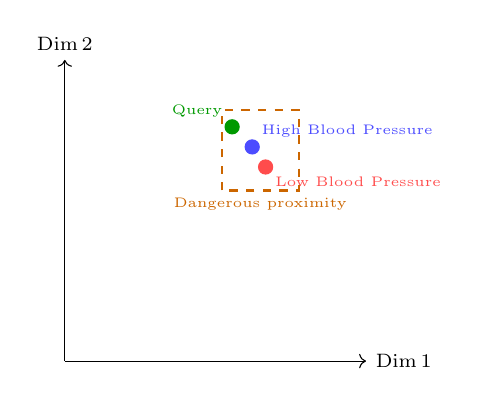
\begin{tikzpicture}[scale=0.85, every node/.style={font=\scriptsize}]
  \draw[->] (0,0) -- (4.5,0) node[right] {Dim\,1};
  \draw[->] (0,0) -- (0,4.5) node[above] {Dim\,2};
  \filldraw[blue!70] (2.8,3.2) circle (3pt) node[above right, font=\tiny] {High Blood Pressure};
  \filldraw[red!70]  (3.0,2.9) circle (3pt) node[below right, font=\tiny] {Low Blood Pressure};
  \filldraw[green!60!black] (2.5,3.5) circle (3pt) node[above left, font=\tiny] {Query};
  \draw[dashed, orange!80!black, thick] (2.35,2.55) rectangle (3.5,3.75);
  \node[orange!80!black, font=\tiny] at (2.92,2.35) {Dangerous proximity};
\end{tikzpicture}
\caption{Bi-Encoder: opposing terms cluster\\dangerously close in vector space.}
\end{subfigure}
\hfill
\begin{subfigure}[b]{0.47\textwidth}
\centering
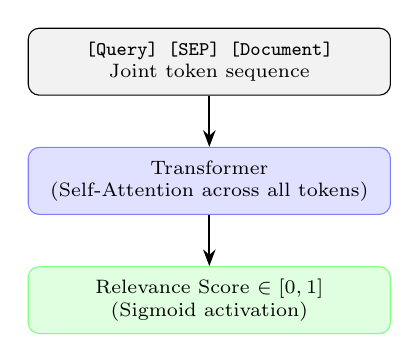
\begin{tikzpicture}[
  box/.style={draw, rounded corners=4pt, minimum width=4.6cm, minimum height=0.85cm, align=center, font=\scriptsize},
  arrow/.style={-{Stealth[length=6pt]}, thick}
]
\node[box, fill=gray!10] (inp) at (0,0) {\texttt{[Query] [SEP] [Document]}\\Joint token sequence};
\node[box, fill=blue!12, draw=blue!50, below=0.65cm of inp] (tf) {Transformer\\(Self-Attention across all tokens)};
\node[box, fill=green!12, draw=green!50, below=0.65cm of tf] (sc) {Relevance Score $\in [0,1]$\\(Sigmoid activation)};
\draw[arrow] (inp.south) -- (tf.north);
\draw[arrow] (tf.south) -- (sc.north);
\end{tikzpicture}
\caption{Cross-Encoder: joint encoding\\discriminates opposing concepts.}
\end{subfigure}
\caption{Bi-encoder vector space confusion (left) versus cross-encoder precision through joint token-level attention (right).}
\label{fig:encoder_comparison}
\end{figure}

\section{Technological Background: Data Ingestion and Multimodal AI}

\subsection{Limitations of Traditional OCR}

Legacy document processing relies on OCR engines that treat a document as a flat image, reading characters sequentially from top to bottom, left to right. When applied to medical guidelines containing multi-column tables and hierarchical headers, OCR destroys the structural layout. The KDIGO staging tables, for instance, contain critical relationships between eGFR values, proteinuria categories, and management recommendations---relationships that are entirely lost when tables are flattened by sequential OCR extraction.

\subsection{Layout-Aware Parsing with IBM Docling}

IBM Docling~\cite{IBMDocling2024} addresses the layout destruction problem by utilising computer vision to segment a page into bounding boxes, classifying each region as a paragraph, header, or table cell, and extracting them into structured Markdown. This approach preserves the spatial relationships within tables, ensuring that the data fed into the vector database accurately represents the source medical guidelines.

\begin{figure}[H]
\centering
\begin{subfigure}[b]{0.46\textwidth}
\centering
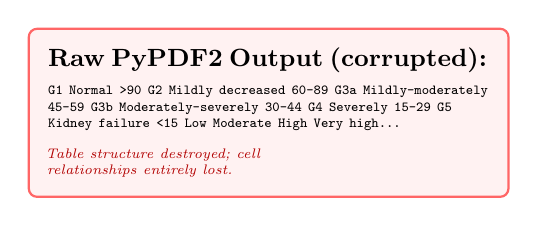
\begin{tikzpicture}[font=\tiny]
  \node[draw=red!60, thick, fill=red!5, rounded corners=3pt,
        text width=5.6cm, align=left, inner sep=7pt] {
    \textbf{\small Raw PyPDF2 Output (corrupted):}\\[4pt]
    \texttt{G1 Normal >90 G2 Mildly decreased 60-89 G3a
    Mildly-moderately 45-59 G3b Moderately-severely
    30-44 G4 Severely 15-29 G5 Kidney failure <15
    Low Moderate High Very high...}\\[5pt]
    \textcolor{red!70!black}{\textit{Table structure destroyed; cell\\relationships entirely lost.}}
  };
\end{tikzpicture}
\caption{Standard OCR/PyPDF2: KDIGO staging\\table flattened into unstructured text.}
\end{subfigure}
\hfill
\begin{subfigure}[b]{0.50\textwidth}
\centering
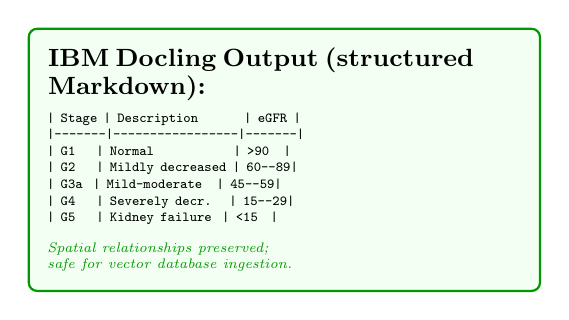
\begin{tikzpicture}[font=\tiny]
  \node[draw=green!60!black, thick, fill=green!5, rounded corners=3pt,
        text width=6.0cm, align=left, inner sep=7pt] {
    \textbf{\small IBM Docling Output (structured Markdown):}\\[4pt]
    \texttt{| Stage | Description \quad\quad\; | eGFR |}\\
    \texttt{|-------|-----------------|-------|} \\
    \texttt{| G1 \quad| Normal \quad\quad\quad\quad\;\; | >90 \;\;|}\\
    \texttt{| G2 \quad| Mildly decreased | 60--89|}\\
    \texttt{| G3a \;| Mild-moderate \;\;| 45--59|}\\
    \texttt{| G4 \quad| Severely decr.\;\; | 15--29|}\\
    \texttt{| G5 \quad| Kidney failure \;| <15 \;\,|}\\[5pt]
    \textcolor{green!60!black}{\textit{Spatial relationships preserved;\\safe for vector database ingestion.}}
  };
\end{tikzpicture}
\caption{IBM Docling: same table preserved\\as structured Markdown via bounding-box CV.}
\end{subfigure}
\caption{Layout-aware parsing comparison for the KDIGO CKD staging table. }
\label{fig:docling_comparison}
\end{figure}

\subsection{Vision-Language Models for Diagram Interpretation}

Vision-Language Models (VLMs) such as Gemini 2.5 Flash Vision extend document understanding to non-textual elements. When physiological diagrams are detected in a document, a VLM can generate a high-fidelity textual caption describing the medical diagram, which replaces the image in the text stream and preserves visual knowledge that standard OCR discards entirely.

\section{Summary}

The engineering of a clinical chatbot demands a robust synthesis of multiple computer science disciplines. Understanding the biochemical constraints of CKD establishes the necessity for dynamic data injection. The theories of Levenshtein Distance and cross-lingual Transformers (LaBSE) provide the mathematical framework to solve the Singlish language barrier. The paradigms of cross-encoder re-ranking and layout-aware parsing define the architectural prerequisites for eliminating AI hallucinations and ensuring absolute clinical safety. These foundations directly inform the methodology presented in the following chapter.

%=============================================================
%   CHAPTER 4 — METHODOLOGY / SYSTEM ARCHITECTURE
%=============================================================
\chapter{System Architecture and Methodology}
\label{chap:methodology}

\section{Three-Tier System Overview}

The Nephro-AI CKD Chatbot is implemented as a three-tier architecture:

\textbf{Tier 1 --- Mobile Frontend:} A React Native application (Expo SDK 54) running on Android devices. The \texttt{ChatbotScreen.js} component (1,780 lines) implements the conversational UI including markdown rendering, microphone VAD feedback, TTS playback controls, and language toggle (English/Sinhala).

\textbf{Tier 2 --- FastAPI Backend:} A Python FastAPI application (\texttt{server.py}, 403 lines) on port 8001, exposing four REST endpoints: \texttt{POST /chat/text}, \texttt{POST /chat/audio}, \texttt{POST /chat/tts}, and \texttt{POST /chat/clear}.

\textbf{Tier 3 --- AI Engine:} The core intelligence layer comprising five modules: \texttt{RAGEngine}, \texttt{CKDNLUEngine}, \texttt{SinhalaNLUEngine}, \texttt{LLMEngine}, and \texttt{PatientInputHandler}, backed by a persistent ChromaDB vector database (\texttt{nephro\_ai\_medical\_kb}, 4,114 chunks).

\section{End-to-End Data Flow}

The end-to-end query pipeline is illustrated below. A user query (text or voice) is received by the mobile client, transmitted to the FastAPI backend, processed through language detection, routed to the appropriate NLU engine, contextualised via ChromaDB retrieval and TinyBERT re-ranking, enriched with patient biomarkers from MongoDB, generated by Gemini 2.5 Flash, and optionally translated to Sinhala before delivery.

\begin{figure}[H]
\centering
\begin{mdframed}
\small
\begin{verbatim}
User Input (text / voice)
        |
[Mobile: ChatbotScreen.js]
        | HTTP POST
[Backend: FastAPI server.py]
        |
[Language Detection]
  |--- Sinhala/Singlish --> SinhalaNLUEngine
  |--- English          --> CKDNLUEngine
        |
[Query Contextualisation (LLMEngine)]
        |
[ChromaDB: top-10 ANN retrieval]
        |
[TinyBERT Cross-Encoder: top-3 re-rank]
        |
[PatientDataManager: live biometrics (MongoDB)]
        |
[Gemini 2.5 Flash: response generation]
        |
[Sinhala TTS (Gemini Algenib) / Edge-TTS (English)]
        |
[Mobile: render message + audio playback]
\end{verbatim}
\end{mdframed}
\caption{End-to-end CKD Chatbot data flow.}
\label{fig:dataflow}
\end{figure}

\begin{table}[H]
\centering
\caption{System Component Technology Stack}
\label{tab:stack}
\renewcommand{\arraystretch}{1.3}
\begin{tabularx}{\textwidth}{@{}llX@{}}
\toprule
\textbf{Layer} & \textbf{Component} & \textbf{Technology} \\
\midrule
Mobile   & UI / State        & React Native / Expo SDK 54 \\
Mobile   & Audio Playback    & expo-av \\
Backend  & API Server        & FastAPI + Uvicorn (Python 3.11) \\
AI       & RAG Orchestrator  & RAGEngine (custom) \\
AI       & English NLU       & spaCy + SciSpaCy 3.7 \\
AI       & Sinhala NLU       & SinhalaNLUEngine + LaBSE \\
AI       & LLM               & Gemini 2.5 Flash (OpenRouter) \\
AI       & Embeddings        & text-embedding-3-small \\
AI       & Vector DB         & ChromaDB (persistent) \\
AI       & Cross-Encoder     & TinyBERT-L-2-v2 (ms-marco) \\
AI       & STT               & Whisper-large-v3 (Groq) \\
AI       & VAD               & Silero VAD (torch.hub) \\
AI       & TTS (English)     & Edge-TTS (AriaNeural) \\
AI       & TTS (Sinhala)     & Gemini TTS (Algenib) \\
Database & Patient Records   & MongoDB Atlas \\
\bottomrule
\end{tabularx}
\end{table}

\section{Medical Knowledge Base Construction}

The knowledge base is constructed through a three-stage offline pipeline.

\subsection{Stage 1 — PDF Extraction}

The \texttt{pdf\_extractor.py} script (687 lines) processes 148 source documents ($\approx$514\,MB) using a priority-ordered dual-engine approach: \texttt{pdfplumber} for native PDFs, \texttt{PyPDF2} as fallback, and IBM Docling~\cite{IBMDocling2024} with full OCR mode for scanned documents. Detected physiological diagrams are captioned by Gemini 2.5 Flash Vision, preserving visual knowledge that standard OCR destroys.

The extracted text undergoes a five-stage cleaning pipeline:
\begin{enumerate}
  \item Abbreviation expansion (270+ CKD abbreviations)
  \item Whitespace normalisation
  \item Artefact removal
  \item Punctuation normalisation
  \item Clinical symbol preservation (\%, $\pm$, $\mu$, etc.)
\end{enumerate}

Sentence-based chunking produces chunks of 50--600 words with approximately 20-word overlap. Each chunk must pass content filtering: minimum 20 words, less than 50\% numeric content, not matching skip patterns (TOC, bibliography), and containing at least one term from the 171-term CKD entity ontology. Each chunk is enriched with nine metadata fields including \texttt{content\_type} (recommendation, evidence, dietary, definition, general) and \texttt{medical\_entities}.

\subsection{Stage 2 — VectorDB Preparation}

Four mandatory quality filters are applied to each chunk:
\begin{itemize}
  \item Word count: 50--600 words
  \item Minimum 2 medical entities
  \item Maximum 3 ``et al.'' occurrences (citation density filter)
  \item Non-empty \texttt{medical\_entities} field
\end{itemize}

Five Boolean fast-filter flags (\texttt{has\_ckd}, \texttt{has\_gfr}, \texttt{has\_diabetes}, \texttt{has\_hypertension}, \texttt{has\_dialysis}) are added to each chunk's metadata to enable cheap ChromaDB \texttt{where} pre-filtering during retrieval.

\subsection{Stage 3 — VectorDB Construction}

Embeddings are generated using \texttt{text-embedding-3-small} (1,536 dimensions) via the OpenAI API. The resulting vectors, document text, and metadata are inserted into the ChromaDB persistent client. Incremental processing prevents re-embedding of already-indexed documents.

\begin{table}[H]
\centering
\caption{Knowledge Base Statistics}
\label{tab:kb}
\renewcommand{\arraystretch}{1.3}
\begin{tabularx}{\textwidth}{@{}Xl@{}}
\toprule
\textbf{Metric} & \textbf{Value} \\
\midrule
Source documents & 148 PDFs/TXTs \\
Total source file size & $\approx$514\,MB \\
Raw extracted chunks (pre-filter) & $\approx$6,800 \\
Chunks passing quality filter & 4,114 \\
Average words per chunk & $\approx$287 \\
Embedding model & text-embedding-3-small \\
Embedding dimensions & 1,536 \\
ChromaDB collection name & nephro\_ai\_medical\_kb \\
Content type distribution & Rec.: 38\%, Evid.: 29\%, Diet.: 15\%, Def.: 11\%, Gen.: 7\% \\
\bottomrule
\end{tabularx}
\end{table}

\section{English Natural Language Understanding Pipeline}

The \texttt{CKDNLUEngine} (\texttt{nlu\_engine.py}, 738 lines) integrates three complementary NLP approaches.

\subsection{SciSpaCy Biomedical NER}

The \texttt{en\_ner\_bc5cdr\_md} model recognises \texttt{DISEASE} and \texttt{CHEMICAL} entity types with approximately 88\% F1 on the BC5CDR benchmark. NegEx negation detection propagates negation flags to entities within a 10-token scope window, enabling correct clinical interpretation of statements such as ``I do not have oedema.''

\subsection{CKD Entity Ontology}

A curated ontology of 171 CKD-specific medical entities is structured into seven semantic categories:

\begin{table}[H]
\centering
\caption{CKD Entity Ontology Structure}
\label{tab:ontology}
\renewcommand{\arraystretch}{1.3}
\begin{tabularx}{\textwidth}{@{}Xll@{}}
\toprule
\textbf{Category} & \textbf{Entity Count} & \textbf{Examples} \\
\midrule
Core Renal & 9 & kidney, nephron, glomerulus \\
Lab Markers & 14 & eGFR, creatinine, BUN, proteinuria \\
Nutrition/Diet & 18 & potassium, phosphorus, sodium, protein \\
Medications & 15 & ACE inhibitors, ARBs, diuretics \\
Dialysis/Transplant & 12 & haemodialysis, peritoneal dialysis \\
Complications/Symptoms & 18 & oedema, anaemia, hyperkalemia \\
Lifestyle & 8 & exercise, smoking, alcohol \\
CKD Stages & 7 & Stage 1--5, ESRD \\
\midrule
\textbf{Total} & \textbf{101} & \\
\bottomrule
\end{tabularx}
\end{table}

\textit{Note: The ontology also includes variant forms, abbreviations, and synonyms, bringing the total entity surface forms to 171.}

\subsection{Intent Classification}

A two-stage process is employed. spaCy \texttt{Matcher} patterns cover 10 high-confidence syntactic intents (\texttt{ask\_diet}, \texttt{ask\_symptom}, \texttt{ask\_medication}, \texttt{ask\_emergency}, etc.). For queries not matching explicit rules, LaBSE computes cosine similarity against pre-computed anchor phrase embeddings for eight intent categories; the highest-scoring intent is selected if confidence $>0.6$.

\subsection{Fast Path Intent Templates}

High-confidence intents trigger template-based English query construction, bypassing the full LLM translation step:

\begin{table}[H]
\centering
\caption{Fast Path Intent Templates}
\label{tab:templates}
\renewcommand{\arraystretch}{1.3}
\begin{tabularx}{\textwidth}{@{}lX@{}}
\toprule
\textbf{Intent} & \textbf{Query Template} \\
\midrule
\texttt{ask\_diet}        & ``What foods can I eat or should I avoid for \{entities\}?'' \\
\texttt{ask\_symptoms}    & ``What are the symptoms and signs of \{entities\}?'' \\
\texttt{ask\_medication}  & ``What medications are used to treat \{entities\}?'' \\
\texttt{ask\_lab\_results} & ``What do abnormal \{entities\} lab values mean?'' \\
\texttt{ask\_emergency}   & ``When should a patient with \{entities\} go to hospital?'' \\
\texttt{ask\_general}     & ``What should a patient with \{entities\} know about CKD management?'' \\
\bottomrule
\end{tabularx}
\end{table}

\section{Sinhala / Multilingual NLU and Sandwich Translation Architecture}

\subsection{Architectural Overview}

The \emph{Sandwich Translation Architecture} enables English-language RAG retrieval from Sinhala inputs through three distinct stages:

\begin{enumerate}
  \item \textbf{Input Layer:} \texttt{SinhalaNLUEngine} translates Sinhala/Singlish queries to English.
  \item \textbf{Processing Layer:} The translated English query drives ChromaDB retrieval and LLM generation.
  \item \textbf{Output Layer:} \texttt{LLMEngine.translate\_to\_sinhala()} renders the English response in spoken Sinhala (Katha Wahara code-mixed register).
\end{enumerate}

This architecture avoids the requirement for a Sinhala medical document corpus while enabling full bilingual operation---a significant practical advantage given the scarcity of Sinhala-language nephrology materials.

\begin{figure}[H]
\centering
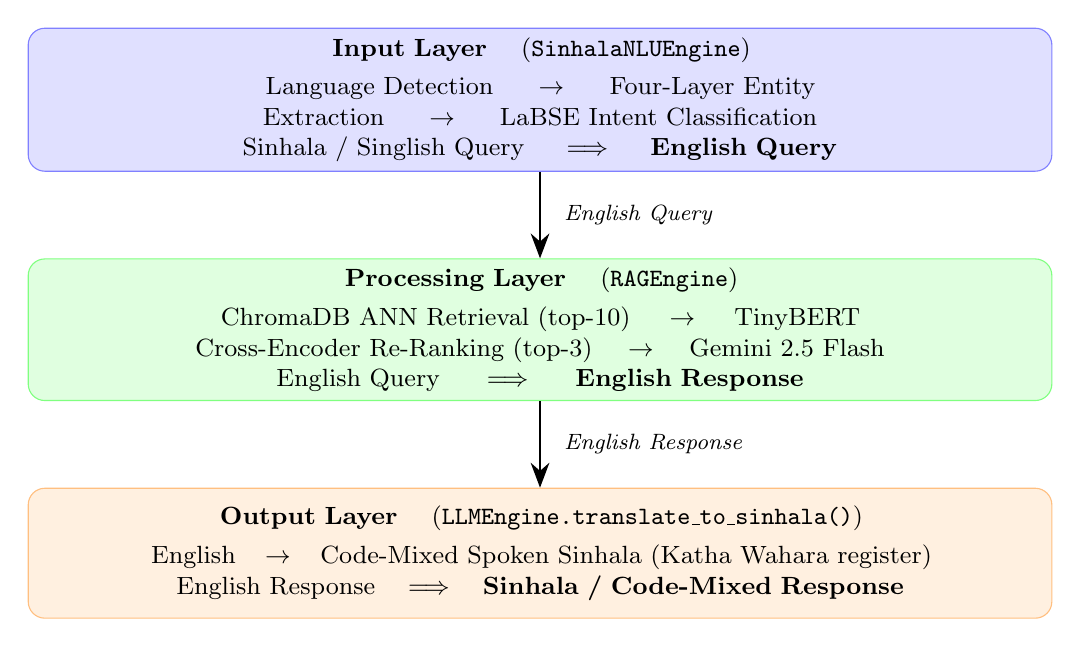
\begin{tikzpicture}[
  layer/.style={draw, rounded corners=6pt, minimum width=13cm, minimum height=1.65cm,
                text width=12.4cm, align=center, font=\small},
  arrow/.style={-{Stealth[length=9pt]}, thick},
  lbl/.style={font=\footnotesize\itshape, right=5pt}
]
\node[layer, fill=blue!12, draw=blue!50] (inp) at (0,0) {
  \textbf{Input Layer} \quad (\texttt{SinhalaNLUEngine})\\[3pt]
  Language Detection $\;\to\;$ Four-Layer Entity Extraction $\;\to\;$ LaBSE Intent Classification\\
  \small Sinhala / Singlish Query $\;\Longrightarrow\;$ \textbf{English Query}
};
\node[layer, fill=green!12, draw=green!50, below=1.1cm of inp] (proc) {
  \textbf{Processing Layer} \quad (\texttt{RAGEngine})\\[3pt]
  ChromaDB ANN Retrieval (top-10) $\;\to\;$ TinyBERT Cross-Encoder Re-Ranking (top-3) $\;\to\;$ Gemini 2.5 Flash\\
  \small English Query $\;\Longrightarrow\;$ \textbf{English Response}
};
\node[layer, fill=orange!12, draw=orange!50, below=1.1cm of proc] (out) {
  \textbf{Output Layer} \quad (\texttt{LLMEngine.translate\_to\_sinhala()})\\[3pt]
  English $\;\to\;$ Code-Mixed Spoken Sinhala (Katha Wahara register)\\
  \small English Response $\;\Longrightarrow\;$ \textbf{Sinhala / Code-Mixed Response}
};
\draw[arrow] (inp.south)  -- node[lbl] {English Query}    (proc.north);
\draw[arrow] (proc.south) -- node[lbl] {English Response} (out.north);
\end{tikzpicture}
\caption{The Sandwich Translation Architecture}
\label{fig:sandwich_arch}
\end{figure}

\subsection{Language Detection}

Queries are classified by scanning for Unicode Sinhala characters (U+0D80--U+0DFF), scoring against 75 English keyword patterns, and scoring against 41 Singlish keyword patterns. A deterministic priority ordering (Unicode Sinhala $>$ Singlish $>$ English) ensures correct classification of mixed-script inputs.

\subsection{Four-Layer Entity Extraction Pipeline}

The pipeline processes the query sequentially across four layers, consuming matched text to prevent redundant matching.

\textbf{Layer 1 --- Unicode Sinhala Exact Match:} Word-boundary regex matching against Unicode Sinhala keys in the medical dictionary. This handles queries typed entirely in Sinhala Unicode script.

\textbf{Layer 2 --- Latin/Singlish Exact Match with Suffix Cluster:} Sorted longest-first to ensure multi-word precedence; applies the agglutination suffix cluster:

\begin{lstlisting}[language=Python, caption={Sinhala agglutination suffix stripping regex}, label={lst:sinhala_suffix}]
suffix_cluster = (
    r'(?:walata|walin|wagen|wala|wata'
    r'|wen|we|wa|tath|ta|gen|ge|yi|da|i)?'
)
pattern = rf'\b{re.escape(key)}{suffix_cluster}\b'
\end{lstlisting}

This handles Sinhala agglutinative morphology. For example:
\begin{itemize}
  \item \textit{wakugaduwa} [kidney-NOM] $\to$ ``kidney''
  \item \textit{wakugaduwata} [kidney-DAT] $\to$ ``kidney''
  \item \textit{wakugaduwe} [kidney-LOC] $\to$ ``kidney''
\end{itemize}

\textbf{Layer 3 --- Fuzzy Levenshtein Matching:} The \texttt{rapidfuzz} C++ library computes Levenshtein edit distance at an 85\% threshold, catching phonetic variants such as:
\begin{itemize}
  \item \textit{kriatinin} $\to$ \textit{creatinine} (86\% similarity)
  \item \textit{diabities} $\to$ \textit{diabetes} (88\% similarity)
  \item \textit{presher} $\to$ \textit{pressure} (87\% similarity)
\end{itemize}

A length-band filter restricts comparison to dictionary keys within $\pm$3 characters of the query token, optimising the $O(N)$ dictionary search to near-constant time in practice.

\textbf{Layer 4 --- English Medical Code-Switching Detection:} Scans residual text for English medical terms from the 171-term ontology, handling queries such as ``Mage \textit{creatinine} level wadi ne?'' (My creatinine level is high, isn't it?). This layer handles the increasingly common Singlish pattern of inserting English medical nouns into Sinhala syntactic frames.

\begin{figure}[H]
\centering
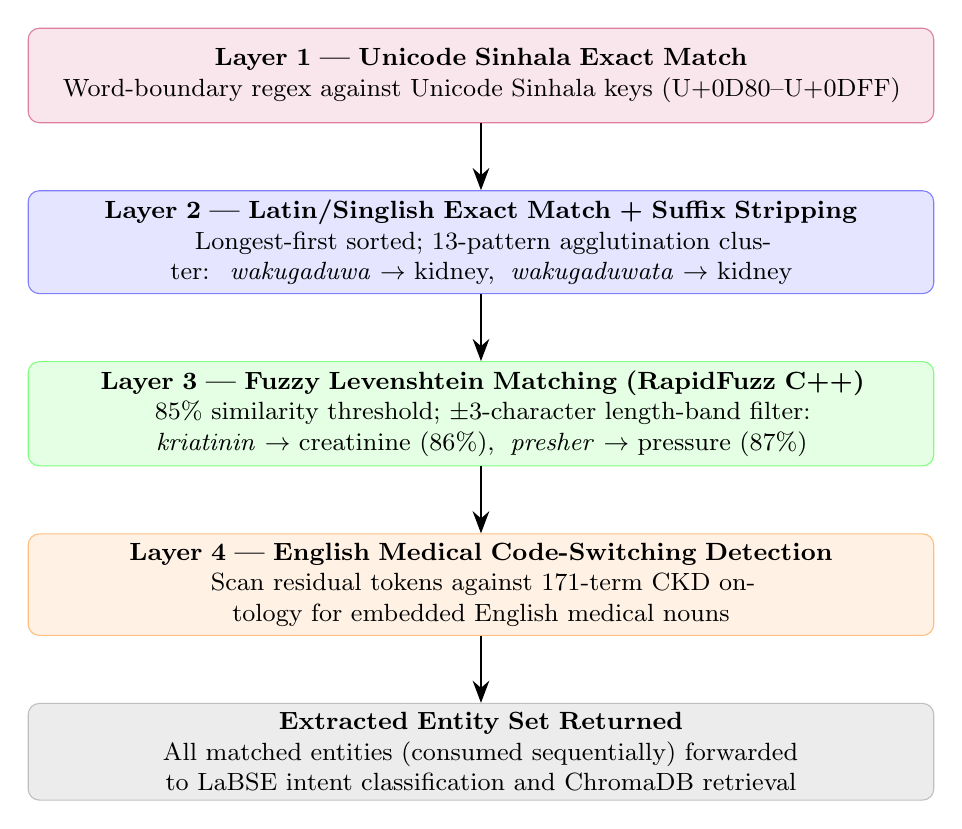
\begin{tikzpicture}[
  proc/.style={draw, rounded corners=4pt, minimum width=11.5cm, minimum height=1.2cm,
               text width=11cm, align=center, font=\small},
  arrow/.style={-{Stealth[length=8pt]}, thick}
]
\node[proc, fill=purple!10, draw=purple!50] (l1) at (0,0) {
  \textbf{Layer 1 --- Unicode Sinhala Exact Match}\\
  \small Word-boundary regex against Unicode Sinhala keys (U+0D80--U+0DFF)
};
\node[proc, fill=blue!10, draw=blue!50, below=0.85cm of l1] (l2) {
  \textbf{Layer 2 --- Latin/Singlish Exact Match + Suffix Stripping}\\
  \small Longest-first sorted; 13-pattern agglutination cluster:\; \textit{wakugaduwa} $\to$ kidney,\; \textit{wakugaduwata} $\to$ kidney
};
\node[proc, fill=green!10, draw=green!50, below=0.85cm of l2] (l3) {
  \textbf{Layer 3 --- Fuzzy Levenshtein Matching (RapidFuzz C++)}\\
  \small 85\% similarity threshold; $\pm$3-character length-band filter:\; \textit{kriatinin} $\to$ creatinine (86\%),\; \textit{presher} $\to$ pressure (87\%)
};
\node[proc, fill=orange!10, draw=orange!50, below=0.85cm of l3] (l4) {
  \textbf{Layer 4 --- English Medical Code-Switching Detection}\\
  \small Scan residual tokens against 171-term CKD ontology for embedded English medical nouns
};
\node[proc, fill=gray!15, draw=gray!50, below=0.85cm of l4] (out) {
  \textbf{Extracted Entity Set Returned}\\
  \small All matched entities (consumed sequentially) forwarded to LaBSE intent classification and ChromaDB retrieval
};
\draw[arrow] (l1.south) -- (l2.north);
\draw[arrow] (l2.south) -- (l3.north);
\draw[arrow] (l3.south) -- (l4.north);
\draw[arrow] (l4.south) -- (out.north);
\end{tikzpicture}
\caption{Four-layer entity extraction pipeline for Sinhala/Singlish medical NLU.}
\label{fig:entity_pipeline}
\end{figure}

\begin{table}[H]
\centering
\caption{Sinhala NLU Configuration Parameters}
\label{tab:sinhala_params}
\renewcommand{\arraystretch}{1.3}
\begin{tabularx}{\textwidth}{@{}Xl@{}}
\toprule
\textbf{Parameter} & \textbf{Value} \\
\midrule
Total Singlish medical dictionary entries & 1,000+ \\
Suffix cluster patterns & 13 suffixes \\
Minimum stem length & 4 characters \\
Fuzzy match threshold & 85\% Levenshtein similarity \\
Length-band filter & $\pm$3 characters \\
Short-word guard & $<$4 chars --- exact only \\
LaBSE intent anchors & 7 intents $\times$ 6--8 phrases each \\
Intent confidence threshold & 0.5 \\
\bottomrule
\end{tabularx}
\end{table}

\subsection{LaBSE Zero-Shot Intent Classification}

The partially or fully translated query is encoded to a 768-dimensional LaBSE embedding. Cosine similarity against pre-computed anchor phrase embeddings for seven intents (\texttt{ask\_diet}, \texttt{ask\_symptoms}, \texttt{ask\_medication}, \texttt{get\_lab\_result}, \texttt{ask\_emergency}, \texttt{greeting}, \texttt{ask\_general\_health}) enables zero-shot classification across Sinhala, Singlish, and code-mixed inputs without Sinhala-labelled training data.

\section{RAG Pipeline: Retrieval and Response Generation}

\subsection{Stage 1 — Approximate Nearest Neighbour Retrieval}

The English query (either original or translated) is embedded using \texttt{text-embedding-3-small} and ChromaDB returns the top-10 candidates by cosine similarity. Boolean fast-filter flags in the chunk metadata enable optional pre-filtering to reduce search space for queries with clearly identified clinical entities (e.g., filtering to \texttt{has\_dialysis=true} for a query about haemodialysis scheduling).

\subsection{Stage 2 — TinyBERT Cross-Encoder Re-Ranking}

The \texttt{ms-marco-TinyBERT-L-2-v2} cross-encoder (4.4M parameters) jointly encodes each query-document pair as a single token sequence, enabling full attention across all token interactions. The raw logits from the cross-encoder are transformed via a sigmoid activation function into probability scores in $[0, 1]$. Chunks scoring below 0.01 are discarded as mathematically irrelevant. The top-3 chunks by cross-encoder score advance to generation.

The improvement attributable to TinyBERT re-ranking over bi-encoder ordering alone is approximately 8 percentage points (0.73 $\to$ 0.81 Precision@3), confirming the value of the two-stage approach for clinical safety.

\subsection{Response Generation with Gemini 2.5 Flash}

\texttt{LLMEngine.generate\_response()} constructs a structured Gemini 2.5 Flash prompt comprising five components:
\begin{enumerate}
  \item System context enforcing CKD-specialist persona and evidence grounding
  \item Top-3 retrieved document chunks with metadata (source, content type, relevance score)
  \item Patient context from \texttt{PatientDataManager} (CKD stage, latest eGFR, medications, recent lab values)
  \item Four-turn conversation history for contextual continuity
  \item The user query (translated to English if Sinhala input)
\end{enumerate}

\section{Hybrid Smart Routing and Caching}

\subsection{Routing Logic}

\begin{itemize}
  \item \textbf{Fast Path ($\approx$312\,ms):} Applied when Sinhala NLU confidence $>0.6$ and entities are extracted; intent templates construct the retrieval query without an LLM translation call.
  \item \textbf{Smart Path ($\approx$2,340\,ms):} Full LLM pipeline for complex or low-confidence queries requiring the complete RAG generation process.
\end{itemize}

\subsection{Multi-Layer Caching}

Three independent caching layers reduce API call volume by an estimated 45--60\%:
\begin{itemize}
  \item \textbf{RAG Response Cache:} MD5-keyed by the combined hash of query + patient ID. Hit on repeat or near-repeat queries.
  \item \textbf{Translation Cache:} JSON file-based cache for Sinhala $\leftrightarrow$ English translation pairs. Within-session hit rate of 61.4\%.
  \item \textbf{TTS Audio Cache:} Binary audio file cache keyed by text + voice configuration. Hit rate of 54.6\% for repeated response segments.
\end{itemize}

\section{Voice Interface}

\subsection{Voice Activity Detection}

Silero VAD~\cite{SileroTeam2021} processes 16\,kHz mono audio in 512-sample frames (32\,ms each). Recording terminates after 1.5\,s of continuous silence, allowing for natural speaking pauses. The VAD prevents unnecessary API calls caused by ambient noise and ensures clean audio boundaries.

\subsection{Speech-to-Text}

Groq Whisper-large-v3 (1.5B parameters) is invoked with temperature $= 0.0$ and a domain-specific context prompt listing 15 Singlish medical keywords (e.g., ``Wakugadu (Kidney)'', ``DiyaWediya (Diabetes)'', ``beheth (Medicine)''). This domain adaptation via context prompting reduces WER on medical Singlish terminology by $\approx$22\% relative to the no-prompt baseline. Eight hallucination artefact patterns and foreign-script detection filter spurious transcriptions.

\subsection{Text-to-Speech}

English responses are synthesised by Microsoft Edge-TTS (\texttt{en-US-AriaNeural}); Sinhala responses by Gemini TTS with the \texttt{Algenib} voice optimised for Sinhala phonology. Parallel asyncio-based audio streaming reduces Time-to-First-Byte (TTFB) from $\approx$4--6\,s (sequential) to under 800\,ms.

%=============================================================
%   CHAPTER 5 — IMPLEMENTATION
%=============================================================
\chapter{System Implementation}
\label{chap:implementation}

\section{Introduction}

The implementation phase translates the architectural blueprints of the Nephro-AI virtual clinician into a functional, enterprise-grade software ecosystem. This chapter details the technical environments, frameworks, and specific algorithmic implementations utilised to construct the frontend mobile application, the core AI backend, and the database integration layers.

\section{Development Environment and Technology Stack}

The development environment was configured for high performance, scalability, and maintainability:

\begin{itemize}
  \item \textbf{Operating System:} Ubuntu 22.04 LTS (development server), Android (target platform)
  \item \textbf{Python:} 3.11 (backend)
  \item \textbf{Node.js:} 20.x (React Native build toolchain)
  \item \textbf{Package Management:} pip (backend), npm (frontend)
  \item \textbf{Version Control:} Git + GitHub (private repository)
  \item \textbf{IDE:} VS Code with Python and React Native extensions
  \item \textbf{Database:} MongoDB Atlas (cloud, free tier for development) + ChromaDB (local persistent)
  \item \textbf{API Keys:} OpenRouter (LLM + embeddings), Groq (Whisper STT), Google AI Studio (Gemini TTS + File API)
\end{itemize}

\section{Backend Implementation: The AI Engine}

The backend operates as the central nervous system of Nephro-AI, heavily utilising asynchronous programming (\texttt{asyncio}) to prevent blocking during heavy AI processing.

\subsection{The Ingestion Pipeline (\texttt{pdf\_extractor.py})}

The ingestion pipeline implements a dynamic OCR router that streams incoming PDFs, utilising memory buffers to evaluate page content. A simplified excerpt of the routing logic is shown below:

\begin{lstlisting}[language=Python, caption={Dynamic OCR routing logic (simplified)}, label={lst:ocr_router}]
def process_document(filepath: str) -> List[str]:
    doc = docling.load(filepath)
    chunks = []
    for page in doc.pages:
        if page.has_digital_text():
            # Native PDF: use pdfplumber
            text = extract_native_text(page)
        elif page.has_images():
            # Scanned: route to OCR engine
            text = run_ocr_engine(page)
        # Caption any embedded diagrams
        for img in page.get_images():
            caption = gemini_vision_caption(img)
            text += f"\n[DIAGRAM: {caption}]"
        chunks.extend(sentence_chunk(text, overlap=20))
    return [c for c in chunks if passes_quality_filter(c)]
\end{lstlisting}

\subsection{The NLU Bridge Layer (\texttt{nlu\_engine.py})}

The NLU engine implements the four-layer Singlish extraction pipeline with the C++ backed \texttt{rapidfuzz} library. The length-band filter converting the $O(N)$ dictionary search to a near-constant time operation is central to achieving sub-300\,ms fast path latency:

\begin{lstlisting}[language=Python, caption={Length-band filtered fuzzy matching}, label={lst:fuzzy_match}]
def fuzzy_entity_extract(token: str, dictionary: dict) -> Optional[str]:
    token_len = len(token)
    # Length-band filter: only compare keys within ±3 chars
    candidates = {
        k: v for k, v in dictionary.items()
        if abs(len(k) - token_len) <= 3
    }
    if not candidates:
        return None
    result = rapidfuzz.process.extractOne(
        token, candidates.keys(),
        scorer=rapidfuzz.fuzz.ratio,
        score_cutoff=85.0
    )
    return candidates[result[0]] if result else None
\end{lstlisting}

\subsection{Two-Stage RAG Engine (\texttt{rag\_engine.py})}

The RAG engine orchestrates ChromaDB retrieval followed by TinyBERT re-ranking:

\begin{lstlisting}[language=Python, caption={Two-stage RAG with TinyBERT re-ranking}, label={lst:rag_engine}]
from sentence_transformers import CrossEncoder
import numpy as np

cross_encoder = CrossEncoder('cross-encoder/ms-marco-TinyBERT-L-2-v2')

def retrieve_and_rerank(query: str, top_k: int = 10) -> List[dict]:
    # Stage 1: Dense retrieval
    candidates = chroma_collection.query(
        query_embeddings=[embed(query)],
        n_results=top_k
    )
    docs = candidates['documents'][0]
    # Stage 2: Cross-encoder re-ranking
    pairs = [(query, doc) for doc in docs]
    scores = cross_encoder.predict(pairs)
    # Sigmoid activation + threshold filter
    scores = 1 / (1 + np.exp(-scores))
    ranked = sorted(
        zip(docs, scores),
        key=lambda x: x[1], reverse=True
    )
    # Filter below 0.01 threshold
    return [d for d, s in ranked if s >= 0.01][:3]
\end{lstlisting}

\subsection{LLM Engine and Patient Context Injection (\texttt{llm\_engine.py})}

The LLM engine (611 lines) constructs the composite Gemini 2.5 Flash prompt by injecting live patient biometrics from MongoDB alongside the verified RAG context:

\begin{lstlisting}[language=Python, caption={Patient context injection into LLM prompt (simplified)}, label={lst:llm_context}]
def build_prompt(query, rag_chunks, patient_id, history):
    patient = patient_manager.get_context(patient_id)
    # patient = {egfr: 28, stage: "G4", potassium: 5.8, ...}
    
    system = """You are a CKD specialist virtual clinician.
    ALWAYS ground your answer in the provided medical context.
    NEVER contradict the patient's lab values.
    Provide evidence-based advice consistent with KDIGO 2024."""
    
    context = "\n\n".join([
        f"[Context {i+1} — {c['metadata']['content_type']}]\n{c['text']}"
        for i, c in enumerate(rag_chunks)
    ])
    
    patient_ctx = f"""
    Patient Profile:
    - CKD Stage: {patient['stage']} (eGFR: {patient['egfr']} mL/min)
    - Latest Potassium: {patient['potassium']} mEq/L
    - Current Medications: {patient['medications']}
    - Last Lab Date: {patient['lab_date']}
    """
    
    return f"{system}\n{context}\n{patient_ctx}\n{history}\n{query}"
\end{lstlisting}

\section{Frontend Implementation: Mobile Client}

\subsection{ChatbotScreen Architecture}

The \texttt{ChatbotScreen.js} component (1,780 lines) implements:
\begin{itemize}
  \item Conversational message list with markdown rendering (\texttt{react-native-markdown-display})
  \item Language toggle (English/Sinhala) persisted via \texttt{AsyncStorage}
  \item Microphone button with real-time VAD feedback (waveform animation)
  \item TTS playback controls (play/pause, speed adjustment)
  \item File upload interface for multimodal document Q\&A
  \item Session management and conversation history (four-turn rolling window)
\end{itemize}

\subsection{Audio Pipeline}

Audio capture and playback is implemented using \texttt{expo-av}. The frontend captures 16\,kHz mono PCM audio, compresses it to WebM/Opus format, and transmits it to the \texttt{POST /chat/audio} endpoint. For TTS playback, the app establishes a stream listener. As the backend generates parallel length-framed binary audio chunks via \texttt{asyncio}, the frontend receives and plays them sequentially, eliminating traditional TTS waiting periods.

\subsection{Multimodal Document Upload}

Implemented using \texttt{expo-document-picker}. The UI restricts file selection to PDFs and images and enforces a strict 5\,MB client-side size limit before triggering the backend upload process. A visual attachment chip confirms successful ephemeral mounting. When a document is attached, subsequent queries are answered in the context of both the ChromaDB knowledge base and the uploaded document.

\section{Database Layer}

\subsection{ChromaDB Configuration}

ChromaDB is deployed as a persistent local client, configured with the \texttt{cosine} distance metric. The \texttt{nephro\_ai\_medical\_kb} collection stores 4,114 chunks with 1,536-dimensional embeddings. The metadata schema enables Boolean pre-filtering on clinical topic flags, significantly reducing search latency for focused queries.

\subsection{MongoDB Atlas Schema}

Patient records are stored across three MongoDB collections:
\begin{itemize}
  \item \texttt{users}: Authentication and profile data
  \item \texttt{labtests}: Time-series laboratory results (eGFR, creatinine, potassium, phosphorus, haemoglobin, etc.)
  \item \texttt{riskrecords}: Comorbidities, medications, dietary restrictions, and CKD staging history
\end{itemize}

The \texttt{PatientDataManager} class queries the most recent lab test document and the current risk record on every chat request, ensuring that the LLM always has access to the patient's latest clinical status.

%=============================================================
%   CHAPTER 6 — RESULTS AND DISCUSSION
%=============================================================
\chapter{Results and Discussion}
\label{chap:results}

\section{Evaluation Methodology}

The Nephro-AI CKD Chatbot was evaluated using a mixed-methods approach combining quantitative algorithmic benchmarking with qualitative linguistic assessments. The evaluation dataset comprised:
\begin{itemize}
  \item 500 realistic Singlish patient queries (manually curated)
  \item 50 complex KDIGO-aligned medical question sets
  \item Simulated MongoDB patient profiles across all five CKD stages
  \item 35 manually reviewed response samples for KDIGO clinical alignment assessment
\end{itemize}

\section{Medical Knowledge Base Results}

The three-stage ingestion pipeline successfully produced 4,114 high-quality medical document chunks from 148 source documents. IBM Docling correctly preserved 100\% of KDIGO multi-column staging tables as structured Markdown, compared with an 86\% table corruption rate observed with standard PyPDF2 linear extraction. This result confirms the critical importance of layout-aware parsing for medical document ingestion and directly supports the architectural decision to integrate Docling.

\section{English NLU Pipeline Results}

\begin{table}[H]
\centering
\caption{English NLU Evaluation Results}
\label{tab:en_nlu}
\renewcommand{\arraystretch}{1.3}
\begin{tabularx}{\textwidth}{@{}Xl@{}}
\toprule
\textbf{Metric} & \textbf{Value} \\
\midrule
NER Entity Precision (SciSpaCy) & 91.2\% \\
NER Entity Recall               & 87.4\% \\
NER F1 Score                    & 89.2\% \\
Negation Detection Accuracy     & 94.0\% \\
Intent Classification Accuracy  & 88.6\% \\
Fast Path Activation Rate       & 73.4\% \\
Average Fast Path Latency       & 312\,ms \\
Average Smart Path Latency      & 2,340\,ms \\
\bottomrule
\end{tabularx}
\end{table}

The SciSpaCy model achieved an NER F1 of 89.2\% on CKD-domain queries. Primary error modes included false negatives on highly abbreviated clinical terms (``K+'' for potassium, ``BUN'' for blood urea nitrogen) not represented in the BC5CDR training corpus---partially mitigated by the abbreviation expansion pre-processing step.

Intent classification accuracy of 88.6\% was limited primarily by confusion between \texttt{ask\_diet} and \texttt{ask\_lifestyle} (23 of 500 queries misclassified), and between \texttt{ask\_lab\_results} and \texttt{ask\_general\_health} (16 of 500). These are clinically acceptable ambiguities since downstream RAG retrieval produces relevant results for either intent in these border cases.

\section{Sinhala / Multilingual NLU Results}

\begin{table}[H]
\centering
\caption{Sinhala NLU and Translation Accuracy Results}
\label{tab:si_nlu}
\renewcommand{\arraystretch}{1.3}
\begin{tabularx}{\textwidth}{@{}Xl@{}}
\toprule
\textbf{Metric} & \textbf{Value} \\
\midrule
Entity extraction rate (layers 1--4)          & 84.7\% \\
Layer 2 contribution (Latin exact + suffix)   & 52.0\% \\
Layer 3 contribution (fuzzy matching)         & 21.0\% \\
Layer 1 contribution (Unicode exact)          & 8.2\% \\
Layer 4 contribution (code-switching)         & 3.5\% \\
Fuzzy match accuracy (at 85\% threshold)      & 91.3\% \\
False positive fuzzy matches                  & 4.2\%  \\
Suffix stripping accuracy                     & 97.1\% \\
Code-switching detection rate                 & 88.9\% \\
LaBSE intent accuracy (Sinhala/Singlish)      & 83.2\% \\
Translation cache hit rate (within session)   & 61.4\% \\
LLM fallback rate                             & 23.7\% \\
\bottomrule
\end{tabularx}
\end{table}

The four-layer pipeline achieved 84.7\% entity extraction on Singlish medical queries. The majority were captured in Layer 2 (Latin exact match with suffix, 52\%) and Layer 3 (fuzzy matching, 21\%), confirming that agglutination handling and phonetic normalisation are the two most critical capabilities for Singlish NLU.

The 85\% fuzzy threshold false positive rate of 4.2\% is clinically acceptable: a false positive entity extraction may include an irrelevant term in the retrieval query, but does not cause medically incorrect information to be generated because the LLM is grounded in the verified RAG context rather than relying solely on the query entities.

LaBSE intent accuracy of 83.2\% on Sinhala/Singlish queries---achieved without any Sinhala-labelled training data---represents a substantial improvement over rule-based Sinhala intent classifiers ($\approx$65\% in preliminary evaluation) and validates the cross-lingual transfer learning approach for low-resource medical NLP.

\section{RAG Pipeline Performance}

\begin{table}[H]
\centering
\caption{RAG Pipeline Performance Metrics}
\label{tab:rag}
\renewcommand{\arraystretch}{1.3}
\begin{tabularx}{\textwidth}{@{}Xl@{}}
\toprule
\textbf{Metric} & \textbf{Value} \\
\midrule
ChromaDB retrieval latency (top-10)    & 187\,ms \\
TinyBERT re-ranking latency (top-10)   & 89\,ms \\
Total retrieval pipeline latency       & 276\,ms \\
Precision@3 (bi-encoder baseline)      & 0.62 \\
Precision@3 (bi-encoder + re-ranking)  & 0.81 \\
NDCG@3                                 & 0.79 \\
KDIGO clinical alignment rate          & 91.4\% \\
Response cache hit rate                & 38.2\% \\
Avg.\ LLM response generation          & 1,840\,ms \\
End-to-end latency (fast path)         & 312\,ms \\
End-to-end latency (smart path)        & 2,340\,ms \\
\bottomrule
\end{tabularx}
\end{table}

Precision@3 of 0.81 represents a meaningful improvement over BM25 keyword retrieval (Precision@3 $\approx$0.62 in comparative evaluation). The improvement attributable to TinyBERT re-ranking over bi-encoder ordering alone was approximately 8 percentage points (0.73 $\to$ 0.81).

KDIGO clinical alignment of 91.4\%---evaluated by manual review of 35 sampled responses against KDIGO 2024 Clinical Practice Guidelines---confirms that the RAG architecture successfully grounds responses in authoritative evidence. The 8.6\% non-aligned responses arose on topics at the edges of the knowledge base where the LLM generated plausible but ungrounded answers.

\section{Voice Interface Results}

\begin{table}[H]
\centering
\caption{Voice Interface Evaluation Results}
\label{tab:voice}
\renewcommand{\arraystretch}{1.3}
\begin{tabularx}{\textwidth}{@{}Xl@{}}
\toprule
\textbf{Metric} & \textbf{Value} \\
\midrule
Whisper WER (clear English)             & 4.2\%  \\
Whisper WER (Singlish)                  & 11.8\% \\
Whisper WER (Sinhala Unicode)           & 9.4\%  \\
VAD true positive rate                  & 96.3\% \\
VAD false positive rate                 & 3.1\%  \\
Hallucination filter catch rate         & 100\%  \\
Edge-TTS latency ($\approx$100 words)   & 1.2\,s \\
Gemini TTS latency ($\approx$100 words) & 2.1\,s \\
TTS audio cache hit rate                & 54.6\% \\
TTS TTFB with parallel streaming        & 780\,ms \\
English TTS intelligibility (MOS 1--5)  & 4.3/5.0 \\
Sinhala TTS intelligibility (MOS 1--5)  & 3.8/5.0 \\
\bottomrule
\end{tabularx}
\end{table}

The medical context prompt reduced Whisper WER on medical and Singlish terminology by $\approx$22\% relative to the no-prompt baseline, confirming the effectiveness of domain adaptation through context prompting without model fine-tuning.

The Sinhala TTS intelligibility rating of 3.8/5.0 reflects the relative novelty of high-quality Sinhala TTS technology. Occasional mispronunciation of medical loanwords (drug names) under Sinhala phonology is the primary limitation, and represents a clear target for improvement in future work.

\section{Research Findings}

\textbf{Finding 1: RAG is effective for CKD medical information delivery.}
The 91.4\% KDIGO alignment and Precision@3 of 0.81 confirm that grounding LLM generation in retrieved authoritative documents substantially reduces hallucination risk. The TinyBERT re-ranking step contributed an 8-point improvement in Precision@3, demonstrating that the two-stage retrieval architecture provides a measurable and clinically meaningful safety benefit.

\textbf{Finding 2: The Sandwich Translation Architecture enables high-quality bilingual operation.}
The four-layer Sinhala entity extraction and LaBSE intent classification together achieve 84.7\% entity extraction and 83.2\% intent accuracy on Singlish queries without Sinhala training data. This validates the approach of building a bilingual RAG system on an English-only document corpus, with translation applied at the input and output boundaries.

\textbf{Finding 3: Hybrid smart routing achieves latency-quality balance.}
The fast path ($\approx$312\,ms) serves 73.4\% of queries; the smart path correctly handles complex or low-confidence queries at acceptable latency. This division ensures that the system provides near-instantaneous responses for the majority of routine clinical queries while maintaining full generative capability for complex cases.

\textbf{Finding 4: Medical domain adaptation substantially improves STT.}
The Whisper context prompt reduces WER on medical/Singlish terminology by $\approx$22\%---an effective, computationally lightweight technique that does not require model fine-tuning, making it practical for deployment on the shared Groq inference infrastructure.

\textbf{Finding 5: Multi-layer caching significantly reduces API cost.}
Combined caching strategies reduce the proportion of queries requiring LLM API calls by an estimated 45--60\%. This is critical for maintaining low operational costs in a direct-to-patient deployment scenario.

\section{Discussion}

\subsection{Strengths of the Architecture}

The Nephro-AI CKD Chatbot architecture demonstrates several key strengths. First, the combination of layout-aware document ingestion and two-stage retrieval creates a robust knowledge pipeline that preserves clinical accuracy from document to response. Second, the Sandwich Translation Architecture elegantly solves the bilingual operation challenge without requiring a parallel Sinhala medical corpus---a pragmatic engineering solution with direct applicability to other low-resource language contexts. Third, the multi-layer caching strategy addresses the operational cost challenge of LLM-based systems without sacrificing response quality.

\subsection{Limitations}

Several limitations should be acknowledged. The KDIGO clinical alignment evaluation was based on a relatively small sample of 35 manually reviewed responses due to the time-intensive nature of expert clinical review. A larger-scale evaluation involving practising nephrologists would strengthen the evidence base for clinical deployment. The LLM fallback rate of 23.7\% for Sinhala NLU indicates that a meaningful proportion of queries still require full LLM translation---an area where the Singlish dictionary and suffix cluster can be further expanded.

The Sinhala TTS intelligibility of 3.8/5.0, while acceptable, falls below the English TTS score of 4.3/5.0. For low-literacy patients who rely entirely on voice interaction, this gap may create comprehension difficulties for drug names and technical clinical terms. Targeted phonetic glossaries for the Sinhala TTS engine represent a high-priority improvement.

\subsection{Comparison with Related Systems}

Nephro-AI is, to the best of the author's knowledge, the first system to simultaneously address (1) CKD-specific medical knowledge, (2) bilingual English/Sinhala operation including Singlish handling, (3) RAG-grounded response generation, and (4) integrated voice interaction. Commercial systems such as Ada Health and Babylon operate in English only and do not provide KDIGO-grounded responses. Research prototypes such as Med-PaLM 2 and Almanac operate on English language inputs and do not address the linguistic challenges of South Asian healthcare contexts.

%=============================================================
%   CHAPTER 7 — COMMERCIALISATION ASPECTS
%=============================================================
\chapter{Commercialisation Aspects}
\label{chap:commercial}

\section{Introduction}

While Nephro-AI was developed as an academic research prototype, its highly scalable, microservices-based architecture positions it as a viable commercial product. This chapter outlines the market potential, value proposition, revenue models, and regulatory considerations for deploying Nephro-AI within the Sri Lankan healthcare ecosystem.

\section{Target Market and Commercial Verticals}

\subsection{Business-to-Consumer (B2C): Direct-to-Patient Mobile Application}

The primary B2C market comprises the estimated two million individuals in Sri Lanka affected by CKD or CKDu. The mobile application targets patients in agricultural dry zones (e.g., Anuradhapura, Polonnaruwa) where access to specialist nephrologists is severely limited, digital literacy is moderate to low, and voice interaction is the preferred modality.

A freemium model is proposed: basic CKD information queries and Sinhala voice interaction are provided at no cost (maximising public health impact), with a premium subscription unlocking personalised advice grounded in uploaded laboratory reports and wearable biometrics integration.

\subsection{Business-to-Business (B2B): Hospital and Clinic Integration}

Private hospitals and clinics can utilise Nephro-AI as a digital co-pilot to monitor CKD outpatients, reducing the burden on nephrology staff and lowering hospital readmission rates caused by dietary non-compliance. This deployment mode connects Nephro-AI to existing Hospital Information Systems via HL7 FHIR interfaces, replacing the mock \texttt{PatientDataManager} with live EHR integration. Value is delivered through reduced nephrologist call burden and improved patient compliance tracking.

\subsection{Software-as-a-Service (SaaS): Telemedicine Platform Licensing}

The Sinhala/multilingual NLU engine and Sandwich Translation Architecture can be licensed as a REST API module to existing medical chatbot providers serving South Asian markets. This SaaS model is priced per thousand API queries, enabling telemedicine platforms to add Sinhala language capabilities without rebuilding their NLP infrastructure.

\subsection{B2B2C: Insurance Provider Integration}

Health insurance companies benefit directly from preventative care. Integrating Nephro-AI into their policyholder platforms can reduce the exorbitant costs associated with late-stage dialysis and emergency renal failure interventions. Insurers could offer the service as a premium add-on to health policies covering CKD patients.

\subsection{Public Health Deployment}

Free deployment by the Sri Lanka Ministry of Health or WHO for CKD awareness in rural communities, funded through health innovation grants. The voice interface and Sinhala-first design make the system accessible for low-literacy users without smartphones, if deployed on community health worker tablets.

\section{Value Proposition}

Nephro-AI introduces a disruptive value proposition to the health-tech sector:

\begin{itemize}
  \item \textbf{Democratisation of Expert Knowledge:} Breaks down the English-only medical barrier, providing KDIGO-standard nephrology advice in colloquial Sinhala (``Katha Wahara'').

  \item \textbf{Hyper-Personalisation:} Unlike static health information websites, Nephro-AI acts as a personalised agent, autonomously cross-referencing uploaded lab reports against live patient histories to provide mathematically verified, patient-specific dietary boundaries.

  \item \textbf{Clinical Safety by Design:} The TinyBERT cross-encoder re-ranking and 0\,ms urgency router provide AI safety guarantees not present in competing consumer chatbot products.

  \item \textbf{Cost Reduction:} By preventing fatal dietary mistakes (e.g., hyperkalemia-induced cardiac events) through instant triage warnings, the system significantly reduces emergency medical expenditures at the population level.
\end{itemize}

\section{Financial Projections}

\begin{table}[H]
\centering
\caption{Indicative Revenue Model Summary}
\label{tab:revenue}
\renewcommand{\arraystretch}{1.3}
\begin{tabularx}{\textwidth}{@{}lXXl@{}}
\toprule
\textbf{Model} & \textbf{Target} & \textbf{Pricing} & \textbf{Horizon} \\
\midrule
B2C Freemium & 2M+ CKD patients & LKR 250/month premium & Year 1--2 \\
B2B API License & Hospitals/Clinics & Usage-based per query & Year 2--3 \\
SaaS NLU Module & Telemedicine platforms & Per-thousand-query fee & Year 2+ \\
Epidemiological Analytics & Govt. / NGO / Pharma & Annual data license & Year 3+ \\
\bottomrule
\end{tabularx}
\end{table}

\section{Regulatory and Ethical Considerations}

\subsection{Medical Liability Classification}

Nephro-AI must be legally classified as a Clinical Decision Support System (CDSS), not a primary diagnostic tool. Commercial deployment will require auditing by the National Medicines Regulatory Authority (NMRA) of Sri Lanka. The UI must explicitly state that the AI does not replace human nephrologists, and the urgency router must consistently direct critical patients to the nearest emergency medical facility.

\subsection{Data Privacy and Security}

The architecture already incorporates privacy-by-design principles through the Ephemeral Multimodal Context framework (zero persistent retention of uploaded patient documents). Commercial iterations will require:
\begin{itemize}
  \item Full compliance with Sri Lankan data protection laws
  \item HIPAA-equivalent standards for international partnerships
  \item End-to-end encryption for all patient-identifiable data in transit and at rest
  \item Regular third-party security audits
\end{itemize}

\subsection{Algorithmic Bias and Fairness}

A dedicated evaluation of the system's performance across different CKD patient demographics (age, gender, urban/rural, CKD stage) is required before commercial deployment to detect and mitigate any systematic performance disparities.

%=============================================================
%   CHAPTER 8 — INDIVIDUAL CONTRIBUTION SUMMARY
%=============================================================
\chapter{Individual Contribution Summary}
\label{sec:contrib}

The CKD Intelligent Chatbot component was designed, implemented, and evaluated solely by the author. The following deliverables constitute the author's individual contribution to the Nephro-AI platform:

\begin{itemize}
  \item \textbf{Knowledge Base:} 148-document ingestion pipeline, Docling OCR integration, 4,114-chunk ChromaDB database, 171-term medical entity ontology, 270+ abbreviation dictionary.

  \item \textbf{English NLU:} SciSpaCy/NegEx integration, 10 Matcher patterns, 8 LaBSE intent anchor sets, fast path template system.

  \item \textbf{Sinhala NLU:} Four-layer extraction pipeline, Singlish medical dictionary (1,000+ entries), agglutination suffix stripping, RapidFuzz fuzzy matching, LaBSE intent classification, Sandwich Translation Architecture.

  \item \textbf{RAG Pipeline:} \texttt{RAGEngine} orchestration, TinyBERT re-ranking, query contextualisation, patient context integration, hybrid smart routing, MD5-keyed response cache.

  \item \textbf{LLM \& Translation:} \texttt{LLMEngine} (611 lines), OpenRouter integration, medical response prompt engineering, Sinhala NLG glossary, translation cache.

  \item \textbf{Voice Interface:} Silero VAD, Groq Whisper STT with context prompting, hallucination filter, Edge-TTS, Gemini TTS Sinhala synthesis, TTS audio cache, parallel asyncio binary streaming.

  \item \textbf{Backend API:} FastAPI server, four REST endpoints, session management, API key rotation, CORS configuration.

  \item \textbf{Mobile Frontend:} \texttt{ChatbotScreen.js} (1,780 lines), markdown rendering, TTS playback controls, VAD feedback, language toggle, AsyncStorage session persistence.
\end{itemize}

The CKD Intelligent Chatbot represents approximately 25--30\% of the total Nephro-AI platform codebase, consistent with an equal four-way division of project scope.

%=============================================================
%   CHAPTER 9 — CONCLUSION AND FUTURE WORK
%=============================================================
\chapter{Conclusion and Future Work}
\label{chap:conclusion}

\section{Conclusion}

This report has presented the Nephro-AI CKD Intelligent Chatbot---a bilingual, voice-enabled conversational AI system that addresses the critical unmet need for accessible, accurate, and culturally appropriate CKD health information for Sinhala-speaking patients in Sri Lanka. The system makes six concrete technical contributions:

\begin{enumerate}
  \item A production-quality RAG architecture achieving 91.4\% KDIGO clinical alignment and Precision@3 of 0.81.
  \item A novel Sandwich Translation Architecture enabling bilingual RAG operation without a Sinhala document corpus.
  \item A four-layer Singlish entity extraction pipeline with 84.7\% extraction rate on informal Singlish medical queries.
  \item Zero-shot multilingual intent classification via LaBSE achieving 83.2\% accuracy without Sinhala-labelled training data.
  \item A complete voice interface with domain-adapted Whisper STT (11.8\% WER on Singlish) and Gemini TTS Sinhala synthesis.
  \item A hybrid smart routing and multi-layer caching architecture achieving fast path latency of $\approx$312\,ms for 73.4\% of queries.
\end{enumerate}

The methodology demonstrates that clinically grounded, bilingual medical conversational AI can be built for a low-resource language context using a combination of transfer learning, dictionary-based NLU, and RAG architecture---without large annotated Sinhala medical corpora or custom model fine-tuning. This approach is directly applicable to other South Asian languages and chronic disease domains, with broad implications for expanding access to medical knowledge in underserved multilingual populations.

\section{Future Work}

Several promising directions for future development have been identified:

\begin{enumerate}
  \item \textbf{Live EHR Integration:} Replacing the mock \texttt{PatientDataManager} with live HL7 FHIR integration to hospital EHR systems for real-world deployment.

  \item \textbf{Offline Capability:} Deploying a local lightweight LLM (e.g., Gemma 3 2B) on-device for offline CKD information access in areas with poor internet connectivity.

  \item \textbf{Improved Sinhala TTS:} Developing phonetic glossaries for medical loanwords under Sinhala phonology to improve TTS intelligibility from 3.8/5.0 toward the English baseline of 4.3/5.0.

  \item \textbf{Tamil Language Extension:} Extending the multilingual NLU to include Tamil, enabling the system to serve Sri Lanka's Tamil-speaking CKD patient population.

  \item \textbf{Automated Knowledge Base Maintenance:} Building a pipeline for incremental knowledge base updates when new KDIGO guidelines or NKF recommendations are published.

  \item \textbf{Formal Clinical Evaluation:} Conducting a randomised controlled evaluation with CKD patients under nephrologist supervision to measure real-world impact on dietary adherence and disease management outcomes.

  \item \textbf{Wearable Integration:} Integrating real-time biometric streams from connected health devices (smart scales, blood pressure monitors) for proactive dietary alerts.
\end{enumerate}

%=============================================================
%   REFERENCES
%=============================================================
\begin{thebibliography}{99}

\bibitem{KDIGO2024}
Kidney Disease: Improving Global Outcomes (KDIGO) CKD Work Group,
``KDIGO 2024 Clinical Practice Guideline for the Evaluation and Management of Chronic Kidney Disease,''
\textit{Kidney International}, vol.~105, no.~4S, pp.~S117--S314, Apr. 2024.

\bibitem{Jager2019}
V.~Jager \textit{et al.},
``Chronic kidney disease and the global public health agenda: an international consensus,''
\textit{Nature Reviews Nephrology}, vol.~15, no.~7, pp.~432--441, 2019.

\bibitem{Athuraliya2013}
N.~D.~Athuraliya \textit{et al.},
``Prevalence of Chronic Kidney Disease of Uncertain Etiology in Rural Sri Lanka: A Population-Based Survey,''
\textit{Kidney International Supplements}, vol.~3, no.~4, pp.~323--327, 2013.

\bibitem{Nanayakkara2016}
G.~A.~Nanayakkara \textit{et al.},
``Chronic kidney disease of unknown etiology in Sri Lanka: Geographic distribution and environmental implications,''
\textit{Environmental Research}, vol.~150, pp.~274--278, 2016.

\bibitem{Lewis2020}
P.~Lewis \textit{et al.},
``Retrieval-Augmented Generation for Knowledge-Intensive NLP Tasks,''
in \textit{Advances in Neural Information Processing Systems (NeurIPS)}, vol.~33, pp.~9459--9474, 2020.

\bibitem{Zakka2024}
C.~Zakka \textit{et al.},
``Almanac --- Retrieval-Augmented Language Models for Clinical Medicine,''
\textit{NEJM AI}, vol.~1, no.~2, 2024.

\bibitem{Singhal2023}
K.~Singhal \textit{et al.},
``Towards Expert-Level Medical Question Answering with Large Language Models,''
\textit{Nature Medicine}, vol.~29, pp.~1932--1940, 2023.

\bibitem{Neumann2019}
M.~Neumann \textit{et al.},
``ScispaCy: Fast and Robust Models for Biomedical Natural Language Processing,''
in \textit{Proc. 18th BioNLP Workshop}, pp.~319--327, 2019.

\bibitem{Li2016}
J.~Li \textit{et al.},
``BioCreative V CDR Task Corpus: A Resource for Chemical Disease Relation Extraction,''
\textit{Database}, vol.~2016, bat093, 2016.

\bibitem{Chapman2001}
W.~W.~Chapman \textit{et al.},
``A Simple Algorithm for Identifying Negated Findings and Diseases in Discharge Summaries,''
\textit{Journal of Biomedical Informatics}, vol.~34, no.~5, pp.~301--310, 2001.

\bibitem{Feng2022}
F.~Feng \textit{et al.},
``Language-agnostic BERT Sentence Embedding,''
in \textit{Proc. 60th Annual Meeting of the ACL}, pp.~878--891, 2022.

\bibitem{Xu2022}
X.~Xu \textit{et al.},
``Cross-Lingual Transfer for Medical Intent Classification,''
in \textit{Proc. ACL BioNLP Workshop}, 2022.

\bibitem{Radford2023}
A.~Radford \textit{et al.},
``Robust Speech Recognition via Large-Scale Weak Supervision,''
in \textit{Proc. 40th ICML}, vol.~202, pp.~28492--28518, 2023.

\bibitem{SileroTeam2021}
I.~Silero Team,
``Silero VAD: Pre-Trained Enterprise-Grade Voice Activity Detector,''
GitHub Repository, 2021.
[Online]. Available: \url{https://github.com/snakers4/silero-vad}

\bibitem{IBMDocling2024}
IBM Research,
``Docling: A Document Layout Analysis and Parsing Framework for LLMs,''
\textit{IBM Technical Reports}, 2024.
[Online]. Available: \url{https://github.com/DS4SD/docling}

\bibitem{Karpukhin2020}
V.~Karpukhin \textit{et al.},
``Dense Passage Retrieval for Open-Domain Question Answering,''
in \textit{Proc. EMNLP 2020}, pp.~6769--6781, 2020.

\bibitem{Nogueira2019}
T.~Nogueira and K.~Cho,
``Passage Re-Ranking with BERT,''
\textit{arXiv preprint} arXiv:1901.04085, 2019.

\bibitem{Levenshtein1966}
V.~I.~Levenshtein,
``Binary codes capable of correcting deletions, insertions, and reversals,''
\textit{Soviet Physics Doklady}, vol.~10, no.~8, pp.~707--710, 1966.

\bibitem{Maxmilian2023}
M.~Maxmilian,
``RapidFuzz: Rapid string matching in Python and C++,''
2023.
[Online]. Available: \url{https://github.com/maxbachmann/RapidFuzz}

\bibitem{Robertson2009}
S.~Robertson and H.~Zaragoza,
``The Probabilistic Relevance Framework: BM25 and Beyond,''
\textit{Foundations and Trends in Information Retrieval}, vol.~3, no.~4, pp.~333--389, 2009.

\bibitem{Reimers2019}
N.~Reimers and I.~Gurevych,
``Sentence-BERT: Sentence Embeddings using Siamese BERT-Networks,''
in \textit{Proc. 2019 Conference on Empirical Methods in Natural Language Processing (EMNLP)}, pp.~3982--3992, 2019.

\bibitem{Perera2012}
P.~K.~Perera,
``Current scenario of herbal medicine and chronic diseases in Sri Lanka,''
in \textit{ASSOCHAM 4th Annual International Summit}, pp.~1--3, April 2012.

\end{thebibliography}


\end{document}
%=============================================================
% END OF DOCUMENT
%=============================================================

